% NEXUS-GO: Master's dissertation defense, version 2, in Brazilian Portuguese.
% Translation of ../v2-colegas/nexus-go-v2.tex with the same frames, order and overlay steps, so that page N here
% is page N there. Numbers follow the English deck (audited against dissertation.tex); tables come from tables.tex
% and the gains chart from gains.tex, both written by gen_pt.py from the English generated files, never by hand.
% Build: latexmk nexus-go-v2-pt.tex (pdfLaTeX + BibTeX; see latexmkrc)
% 04/11: advisor's annotations applied (RELATORIO-BEAMER.md); frames no longer match the English deck page by page.
\documentclass[aspectratio=169,11pt]{beamer}
\usetheme{Madrid}
\usepackage[T1]{fontenc}
\usepackage[utf8]{inputenc}
\usepackage[english,brazilian]{babel}
\usepackage{lmodern}
\usepackage{amsmath,amssymb}
\usepackage{booktabs}
\usepackage{appendixnumberbeamer}
\usepackage{tikz}
\usetikzlibrary{positioning,arrows.meta,fit,shadows,babel}
\graphicspath{{figures/}{logos/}}

% ---- colours: navy title bar and footline (Wilson), light blocks (Juliana) ---------------------
\definecolor{navy}{HTML}{0D3366}
\definecolor{midblue}{HTML}{03506F}
\definecolor{greyblue}{HTML}{668CA6}
\definecolor{blockhead}{HTML}{CCDCEE}
\definecolor{blockbody}{HTML}{F5F8FC}
\definecolor{answerhead}{HTML}{D6CEF0}
\definecolor{answerbody}{HTML}{F2EEFA}
\definecolor{eqbg}{HTML}{F7F7FC}
\definecolor{accent}{HTML}{9B1B30}
\definecolor{seq}{HTML}{2B6CB0}
\definecolor{net}{HTML}{C05621}
\definecolor{fus}{HTML}{2F855A}

\setbeamercolor{structure}{fg=navy}
\setbeamercolor{normal text}{fg=black}
\setbeamercolor{frametitle}{bg=navy, fg=white}
\setbeamercolor{title}{bg=navy, fg=white}
\setbeamercolor{author in head/foot}{bg=greyblue, fg=white}
\setbeamercolor{title in head/foot}{bg=midblue, fg=white}
\setbeamercolor{date in head/foot}{bg=navy, fg=white}
\setbeamercolor{block title}{bg=blockhead, fg=black}
\setbeamercolor{block body}{bg=blockbody, fg=black}
\setbeamercolor{block title alerted}{bg=answerhead, fg=black}
\setbeamercolor{block body alerted}{bg=answerbody, fg=black}
\setbeamercolor{alerted text}{fg=accent}
\setbeamercolor{caption name}{fg=navy}
\setbeamercolor{eqbox}{bg=eqbg, fg=black}
\setbeamercolor{bibliography entry author}{fg=black}
\setbeamercolor{bibliography entry title}{fg=black}
\setbeamercolor{bibliography entry location}{fg=black}
\setbeamercolor{bibliography entry note}{fg=black}

% ---- layout: no headline, full-width title bar, numbered captions and outline ---------------
\setbeamertemplate{navigation symbols}{}
\setbeamertemplate{headline}{}
\setbeamertemplate{frametitle}{%
  \nointerlineskip
  \begin{beamercolorbox}[wd=\paperwidth, ht=0.72cm, dp=0.33cm, leftskip=0.45cm]{frametitle}%
    \usebeamerfont{frametitle}\insertframetitle
  \end{beamercolorbox}\vspace{0.15cm}}
\setbeamerfont{frametitle}{size=\Large}
\setbeamertemplate{itemize items}[circle]
\setbeamertemplate{section in toc}[sections numbered]
\setbeamerfont{section in toc}{size=\large}
\setbeamertemplate{caption}[numbered]
\setbeamerfont{caption}{size=\scriptsize}
% references as numbered, run-in entries (one paragraph each)
\setbeamertemplate{bibliography item}[text]
\setbeamertemplate{bibliography entry title}{}
\setbeamertemplate{bibliography entry location}{}
\setbeamertemplate{bibliography entry note}{}
\setbeamersize{text margin left=0.6cm, text margin right=0.6cm}

\AtBeginSection[]{\begin{frame}\vfill\tableofcontents[currentsection]\vfill\end{frame}}

% equation box with a shadow (Wilson's metric slides)
\newenvironment{eqbox}[1][0.8\textwidth]%
  {\begin{center}\begin{beamercolorbox}[rounded=true, shadow=true, wd=#1, sep=4pt, center]{eqbox}}%
  {\end{beamercolorbox}\end{center}}
% callout that appears on a later overlay next to a table (Wilson's result slides)
\newcommand{\nohyphens}{\hyphenpenalty=10000\exhyphenpenalty=10000\relax}
\tikzset{callout/.style={draw=navy, line width=0.6pt, fill=white, rounded corners=2pt, align=left, inner sep=6pt,
  font=\small\nohyphens, drop shadow={opacity=0.3}}}
\newcommand{\callout}[1]{\tikz\node[callout, text width=0.86\linewidth]{#1};}
% highlight of one part of a diagram (Wilson's methodology walkthrough); overlay: the diagram never moves
\tikzset{hl/.style={draw=red!75!black, very thick, rounded corners=3pt, inner sep=4pt, overlay}}

\newcommand{\wF}{wF_{\max}}
\newcommand{\Smin}{S_{\min}}
\newcommand{\NX}[1]{\textsc{nexus-go}/#1}
% generated by gen_pt.py from ../v2-colegas/tables.tex (gen_tables.py, data/thesis_tables.json); do not edit

% tab:cafa5
\newcommand{\TabCorpus}{%
\begin{tabular}{lrrrr}\toprule
Ontologia & Treinamento & Validação & Teste & Termos \\ \midrule
Processo Biológico (BP) & 73.768 & 9.221 & 9.221 & {500} \\
Componente Celular (CC) & {74.328} & {9.292} & {9.292} & 498 \\
Função Molecular (MF) & 62.909 & 7.864 & 7.864 & 499 \\
\bottomrule\end{tabular}}

% tab:gnn_gcn_gat
\newcommand{\TabGNN}{%
\begin{tabular}{llrrrr}\toprule
Codificador de grafos & Cabeça & BP & CC & MF & Média \\ \midrule
GCN (2 camadas) & Vetorial & \textbf{55,78} & \textbf{66,35} & \textbf{67,83} & \textbf{63,32} \\
 & Visual & 53,10 & 63,33 & 65,46 & 60,63 \\
GAT (2 camadas, 4 cabeças) & Vetorial & 46,47 & 61,14 & 63,83 & 57,15 \\
 & Visual & 46,17 & 59,45 & 61,03 & 55,55 \\
\bottomrule\end{tabular}}

% tab:late_fusion
\newcommand{\TabLate}{%
\begin{tabular}{lrrrr}\toprule
Regra de combinação & BP & CC & MF & Média \\ \midrule
Interpolação linear ($\gamma$) & \textbf{57,96} & \textbf{68,79} & \textbf{74,44} & \textbf{67,06} \\
Máximo & 57,35 & 67,79 & 72,59 & 65,91 \\
Mínimo & 56,38 & 68,09 & 72,69 & 65,72 \\
Sigmoide de IC & 57,03 & 67,57 & 73,88 & 66,16 \\
Sigmoide de grau & 57,02 & 67,76 & 72,42 & 65,73 \\
Equação mestra & 57,42 & 68,10 & 73,93 & 66,48 \\
\textit{Stacking} (árvore de decisão) & 56,22 & 67,35 & 73,76 & 65,78 \\
\textit{Stacking} (reg. logística) & 57,53 & 68,50 & 72,47 & 66,17 \\
\textit{Stacking} (MLP) & 56,92 & 68,12 & 73,92 & 66,32 \\
\textit{Stacking} (floresta aleatória) & 56,65 & 68,21 & 74,14 & 66,33 \\
\textit{Stacking} (\textit{gradient boosting}) & 56,67 & 67,72 & 74,18 & 66,19 \\
\bottomrule\end{tabular}}

% tab:vetor_visao_ontologia
\newcommand{\TabVV}{%
\begin{tabular}{llrrrr}\toprule
Etapa & Cabeça & BP & CC & MF & Média \\ \midrule
Primeira Geração & Vetorial & 36,37 & 48,25 & 48,92 & 44,51 \\
 & Visual & 30,40 & 40,84 & 42,42 & 37,89 \\
Propagação fixa & Vetorial & 55,23 & 66,94 & 73,18 & 65,12 \\
 & Visual & 52,17 & 63,06 & 68,25 & 61,16 \\
GNN de ponta a ponta & Vetorial & 55,78 & 66,35 & 67,83 & 63,32 \\
 & Visual & 53,10 & 63,33 & 65,46 & 60,63 \\
Fusão precoce & Vetorial & \textbf{56,52} & \textbf{67,20} & \textbf{73,81} & \textbf{65,84} \\
 & Visual & 53,17 & 64,77 & 69,52 & 62,49 \\
\bottomrule\end{tabular}}

% tab:confronto_bp
\newcommand{\TabTestBP}{%
\begin{tabular}{lrrrrrr}\toprule
Método & $F_{\max}$ & $F^{*}_{\max}$ & $wF_{\max}$ & AuPRC & IAuPRC & $S_{\min}\downarrow$ \\ \midrule
\textit{Baseline} ingênuo & 44,26 & 42,23 & 40,22 & 40,42 & 37,28 & 22,28 \\
DeepGraphGO & 55,29 & 52,21 & 48,92 & 54,04 & 57,89 & 20,11 \\
SEGT-GO & 52,05 & 48,22 & 44,57 & 42,82 & 50,71 & 21,24 \\
Mashup & 43,58 & 41,86 & 39,64 & 34,82 & 32,57 & 23,22 \\
MELISSA & 41,94 & 40,08 & 37,72 & 32,72 & 31,17 & 23,42 \\
deepNF & 35,59 & 31,14 & 26,95 & 34,15 & 33,66 & 25,73 \\ \midrule
Primeira Geração & 46,25 & 39,86 & 37,30 & 45,57 & 47,37 & 23,68 \\
\textit{Baseline} ProtT5 & 59,61 & 56,31 & 53,74 & 58,53 & 62,92 & 18,92 \\ \midrule
NEXUS-GO/Fixed & 61,27 & 58,13 & 55,61 & 60,39 & 65,09 & 18,30 \\
NEXUS-GO/GNN & 62,05 & 59,17 & 56,95 & 60,97 & 66,27 & 17,66 \\
NEXUS-GO/Early & 62,87 & 59,81 & 57,51 & 62,42 & 65,73 & 17,35 \\
NEXUS-GO/Late & \textbf{63,74} & \textbf{60,96} & \textbf{58,69} & \textbf{64,02} & \textbf{68,83} & \textbf{17,12} \\
\bottomrule\end{tabular}}

% tab:confronto_cc
\newcommand{\TabTestCC}{%
\begin{tabular}{lrrrrrr}\toprule
Método & $F_{\max}$ & $F^{*}_{\max}$ & $wF_{\max}$ & AuPRC & IAuPRC & $S_{\min}\downarrow$ \\ \midrule
\textit{Baseline} ingênuo & 58,43 & 56,52 & 48,13 & 56,26 & 51,22 & 10,84 \\
DeepGraphGO & 73,74 & 71,11 & 60,35 & 71,88 & 78,59 & 9,67 \\
SEGT-GO & 71,18 & 68,07 & 55,52 & 63,24 & 74,74 & 10,42 \\
Mashup & 59,37 & 57,44 & 48,28 & 51,27 & 50,30 & 11,06 \\
MELISSA & 58,54 & 56,51 & 47,19 & 49,78 & 48,97 & 11,23 \\
deepNF & 62,49 & 57,59 & 36,51 & 58,44 & 65,10 & 13,52 \\ \midrule
Primeira Geração & 67,38 & 63,46 & 48,39 & 63,83 & 72,20 & 12,03 \\
\textit{Baseline} ProtT5 & 76,79 & 74,29 & 64,78 & 73,30 & 82,06 & 9,47 \\ \midrule
NEXUS-GO/Fixed & 78,20 & 75,85 & 66,93 & 74,32 & 83,78 & 8,85 \\
NEXUS-GO/GNN & 78,42 & 76,01 & 66,70 & 74,41 & 84,07 & 8,44 \\
NEXUS-GO/Early & 78,42 & 76,02 & 67,18 & 74,33 & 83,72 & 8,57 \\
NEXUS-GO/Late & \textbf{79,72} & \textbf{77,52} & \textbf{69,02} & \textbf{76,73} & \textbf{86,26} & \textbf{8,22} \\
\bottomrule\end{tabular}}

% tab:confronto_mf
\newcommand{\TabTestMF}{%
\begin{tabular}{lrrrrrr}\toprule
Método & $F_{\max}$ & $F^{*}_{\max}$ & $wF_{\max}$ & AuPRC & IAuPRC & $S_{\min}\downarrow$ \\ \midrule
\textit{Baseline} ingênuo & 52,54 & 48,26 & 43,38 & 49,41 & 45,93 & 8,46 \\
DeepGraphGO & 76,98 & 73,14 & 68,96 & 74,03 & 80,41 & 5,67 \\
SEGT-GO & 73,40 & 68,76 & 64,12 & 58,64 & 75,15 & 6,37 \\
Mashup & 54,52 & 49,82 & 44,22 & 47,87 & 47,29 & 8,30 \\
MELISSA & 53,57 & 48,65 & 42,86 & 46,43 & 46,31 & 8,47 \\
deepNF & 58,43 & 48,70 & 39,00 & 54,55 & 53,49 & 9,36 \\ \midrule
Primeira Geração & 61,04 & 53,38 & 48,62 & 49,34 & 62,42 & 9,20 \\
\textit{Baseline} ProtT5 & 79,75 & 76,02 & 72,57 & 73,75 & 82,25 & 5,31 \\ \midrule
NEXUS-GO/Fixed & 79,75 & 76,02 & 72,57 & 73,75 & 82,25 & 5,31 \\
NEXUS-GO/GNN & 76,09 & 71,74 & 67,77 & 67,50 & 80,64 & 6,04 \\
NEXUS-GO/Early & 80,22 & 76,54 & 72,94 & \textbf{81,88} & 82,05 & 5,22 \\
NEXUS-GO/Late & \textbf{80,89} & \textbf{77,41} & \textbf{73,89} & 76,53 & \textbf{84,92} & \textbf{5,14} \\
\bottomrule\end{tabular}}

% tab:custo
\newcommand{\TabCost}{%
\begin{tabular}{lrrrrrr}\toprule
Família (rota + cabeça) & Execuções & s/época & h/execução & h totais & VRAM (GiB) & Épocas \\ \midrule
Propagação fixa + vetorial & 49 & \textbf{5,24} & 0,35 & 15,1 & \textbf{6,4} & 250 \\
Propagação fixa + visual & 26 & 18,45 & 0,17 & 4,5 & \textbf{6,4} & 35 \\
GNN de ponta a ponta + vetorial & 6 & 102,14 & 6,09 & 38,7 & 20,7 & 213 \\
GNN de ponta a ponta + visual & 6 & 108,41 & 4,35 & 31,3 & 21,1 & 138 \\
Fusão precoce + vetorial & 40 & 5,26 & 0,27 & 10,2 & \textbf{6,4} & 205 \\
Fusão precoce + visual & 20 & 18,63 & \textbf{0,16} & 3,2 & \textbf{6,4} & 30 \\
\bottomrule\end{tabular}}

% tab:degree_graph_gain
\newcommand{\TabGain}{%
\begin{tabular}{lrrr}\toprule
Grau & BP & CC & MF \\ \midrule
0 (isoladas) & +3,24 [h] & +1,66 [f] & +0,21 [h] \\
1--2 & +1,68 [h] & +2,18 [f] & +0,24 [h] \\
3--5 & +1,77 [f] & +2,31 [f] & $-$0,33 [h] \\
6--14 & +3,79 [h] & +2,44 [h] & +1,06 [h] \\
15--49 & +5,97 [h] & +4,01 [g] & +1,73 [h] \\
$\geq$ 50 & +9,05 [h] & +8,71 [g] & +4,64 [h] \\
\bottomrule\end{tabular}}

% tab:cobertura
\newcommand{\TabCov}{%
\begin{tabular}{lrrr}\toprule
Família de métodos & BP (\%) & CC (\%) & MF (\%) \\ \midrule
DeepGraphGO / SEGT-GO & 96,3 & 95,1 & 95,7 \\
Mashup / MELISSA / deepNF & 63,6 & 66,6 & 68,7 \\
Este trabalho (todas as rotas) & 100,0 & 100,0 & 100,0 \\
\bottomrule\end{tabular}}

% generated by gen_pt.py from ../v2-colegas/gains.tex (gen_gains.py, data/thesis_tables.json); do not edit
\newcommand{\GainBars}{1/43.56/gray/Ingênuo/43{,}56, 2/44.51/net/Ger.~1/44{,}51, 3/63.92/seq/Só ProtT5/63{,}92, 4/63.32/net/GNN/63{,}32, 5/65.12/net/Fixed/65{,}12, 6/65.84/fus/Early/65{,}84, 7/67.06/fus/Late/67{,}06}


% the dissertation has no Portuguese title, so the cover keeps the official English one
\title[Defesa de Mestrado]{NEXUS-GO: Network-Extended Unified Sequence Embeddings\\for Gene Ontology Function Annotation}
\author[Yeonatan Mauhnoom]{Yeonatan Mauhnoom}
\institute[IC/Unicamp]{Orientador: Prof.\ Dr.\ Zanoni Dias\\
  Coorientadores: Prof.\ Dr.\ Hélio Pedrini e Dr.\ Gabriel Bianchin de Oliveira\\[0.9em]
  Instituto de Computação, Universidade Estadual de Campinas (Unicamp)}
\date[16 de novembro de 2026]{16 de novembro de 2026}
\hypersetup{pdftitle={NEXUS-GO: defesa de mestrado}, pdfauthor={Yeonatan Mauhnoom}}

\begin{document}

\begin{frame}
  \titlepage
\end{frame}

\begin{frame}{Sumário}
  \tableofcontents
\end{frame}

% =================================================================================== Introduction
\section{Introdução}

\begin{frame}{Motivação e Contexto}
  \begin{itemize}\setlength{\itemsep}{0.55em}
    \item \textbf{Proteínas:} participam de quase todos os processos celulares, da catálise à sinalização e ao
      transporte.
    \item \textbf{A lacuna:} as bases de sequências crescem rápido, enquanto a caracterização experimental é lenta e
      cara~\cite{dessimoz_cafa_2013}.
    \item \textbf{Predição automática:} métodos de aprendizado de máquina tentam reduzir essa lacuna, avaliados pelo
      desafio CAFA~\cite{dessimoz_cafa_2013}.
    \item \textbf{Evidência complementar:} as redes de interação trazem o contexto de vias e complexos, que a sequência
      sozinha pode não recuperar~\cite{vazquez_global_2003}.
  \end{itemize}
  \vspace{0.6em}
  Este trabalho combina as duas fontes: \textit{embeddings} de um modelo de linguagem de proteínas e a rede STRING.
\end{frame}

\begin{frame}{Função como Hierarquia de Termos}
  \begin{columns}[c]
    \column{0.44\textwidth}
    \begin{itemize}\setlength{\itemsep}{0.4em}
      \item \textbf{\textit{Gene Ontology}:} Processo Biológico (BP), Componente Celular (CC) e Função Molecular
        (MF)~\cite{ashburner_gene_2000}
      \item Cada ontologia é um grafo acíclico dirigido de termos (\texttt{is\_a}, \texttt{part\_of})
      \item \textbf{\textit{True Path Rule}:} um termo implica todos os seus ancestrais~\cite{valentini2010true}
      \item \textbf{Tarefa:} classificação hierárquica multirrótulo
    \end{itemize}
    \column{0.54\textwidth}
    \begin{figure}
      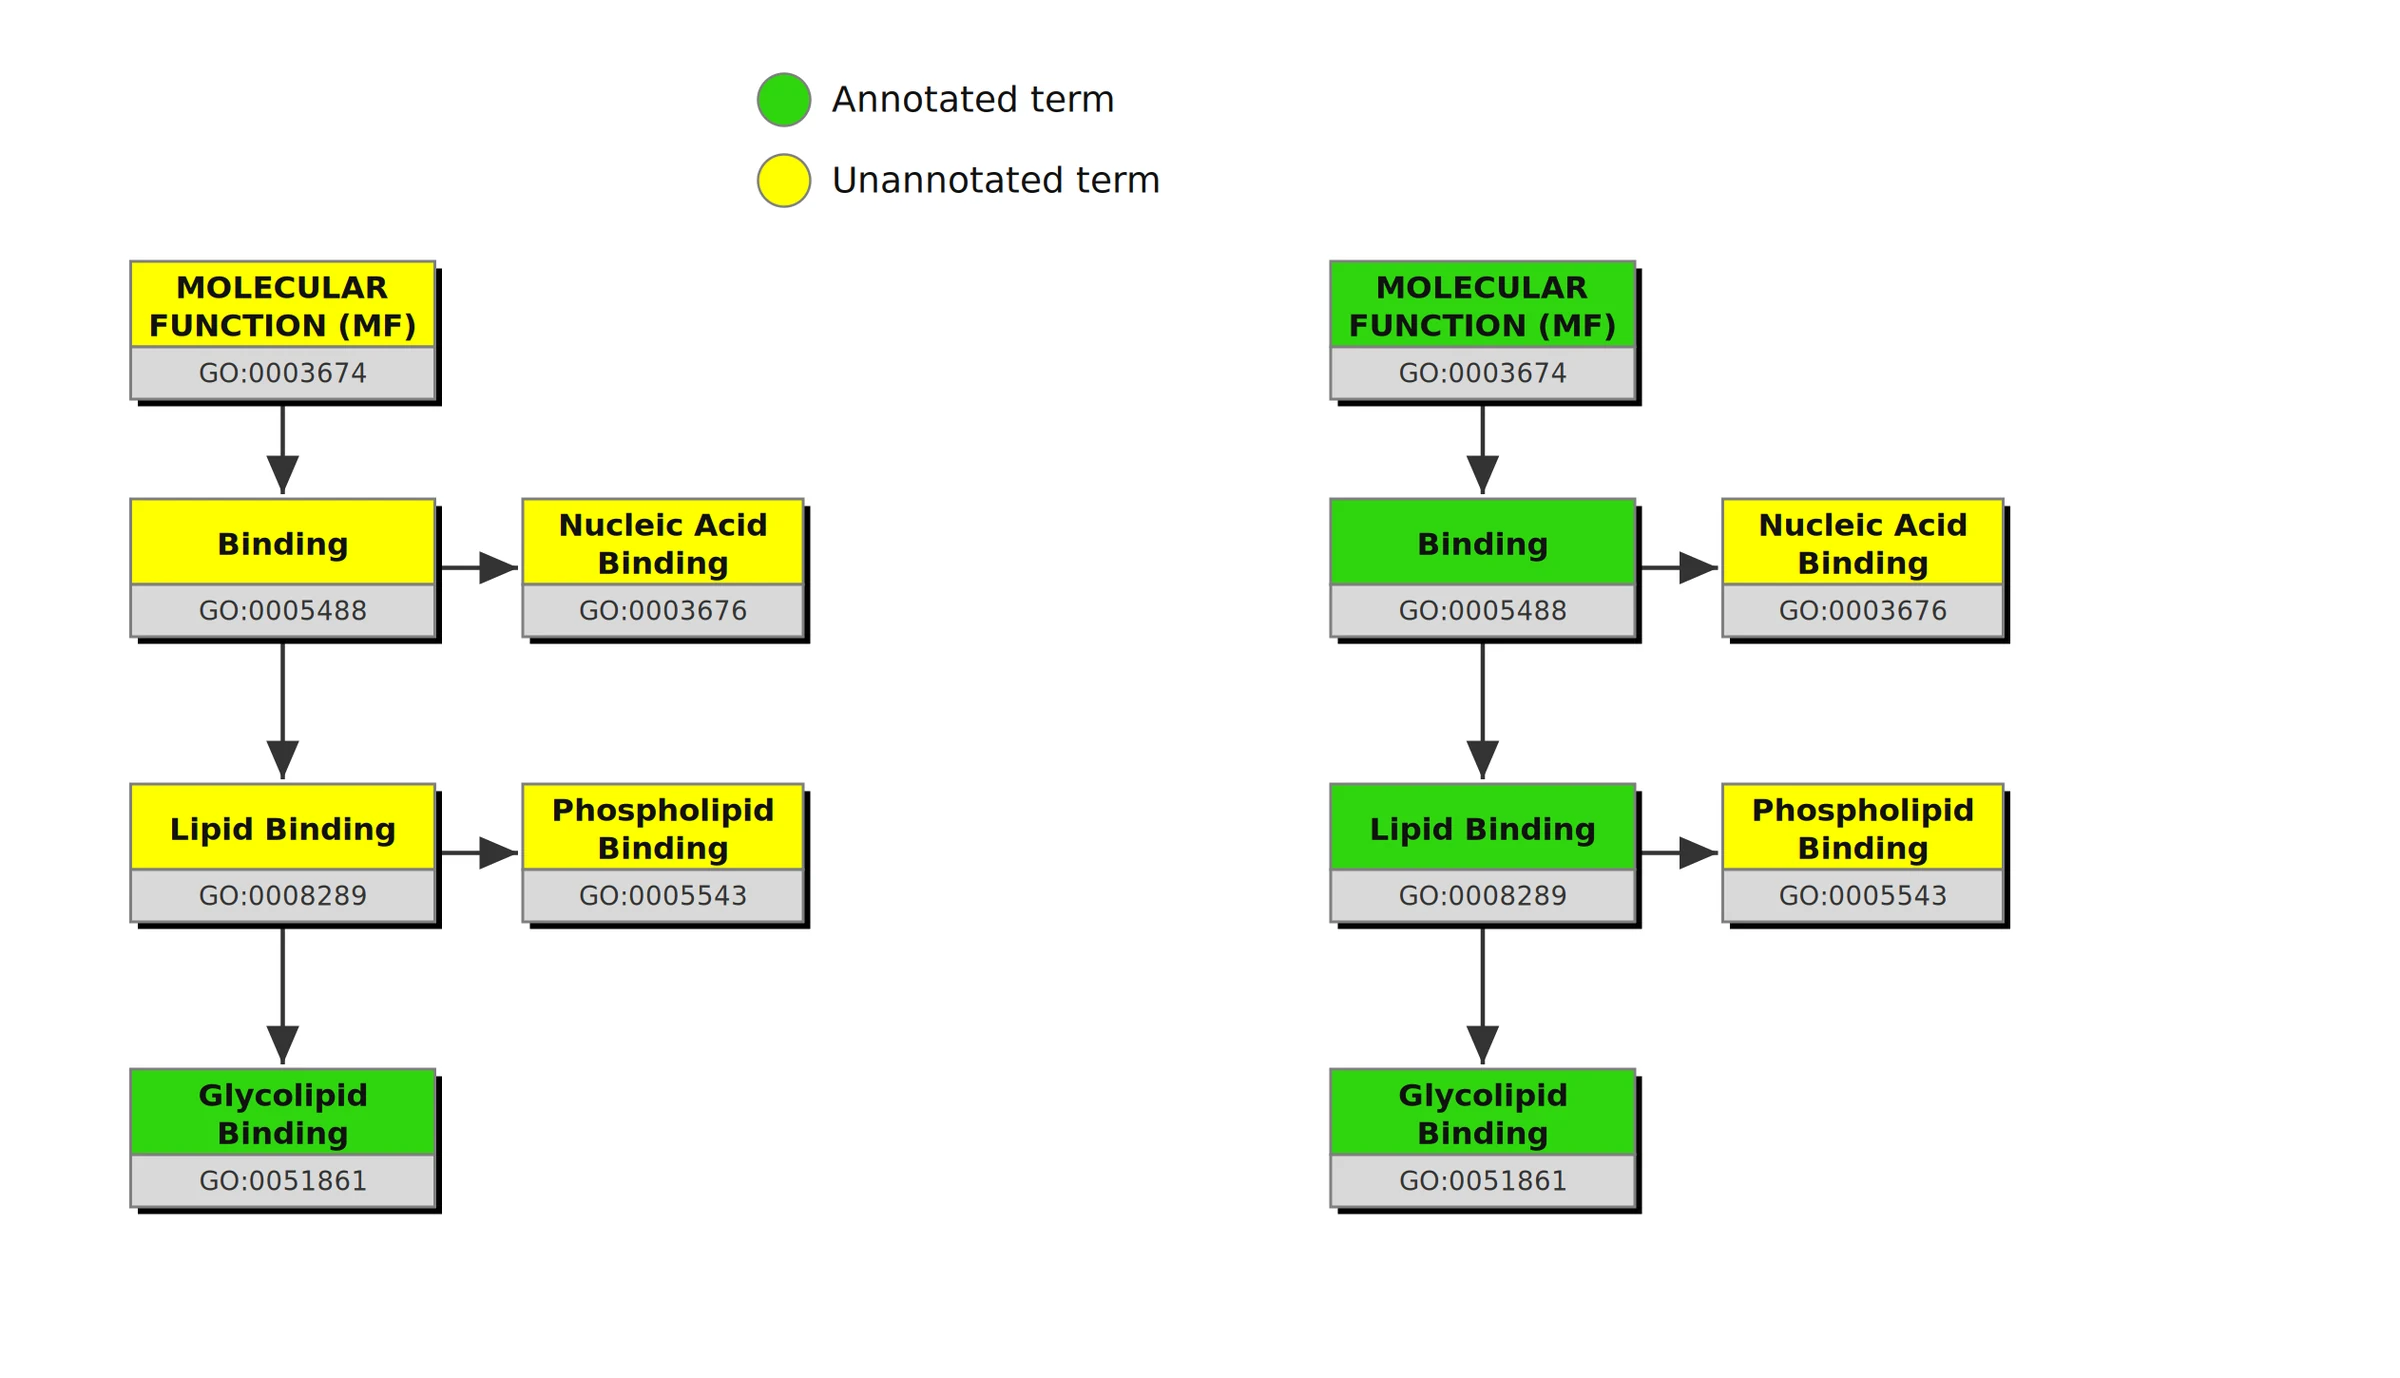
\includegraphics[width=\linewidth]{fig_2_1}
      \caption{Anotação inconsistente (esquerda) e consistente (direita).}
    \end{figure}
  \end{columns}
\end{frame}

\begin{frame}{A Função Também Depende do Contexto}
  \begin{columns}[c]
    \column{0.6\textwidth}
    \begin{itemize}\setlength{\itemsep}{0.4em}
      \item Proteínas atuam em complexos e vias
      \item \textbf{Redes de interação de proteínas (PPI):} os nós são proteínas, e as arestas, associações
      \item \textbf{Culpa por associação:} proteínas conectadas tendem a compartilhar
        funções~\cite{vazquez_global_2003}
      \item O STRING mistura canais de evidência de confiabilidade desigual~\cite{szklarczyk_string_2021}
      \item Cerca de um terço das proteínas não tem nenhuma aresta
    \end{itemize}
    \column{0.36\textwidth}
    \begin{figure}
      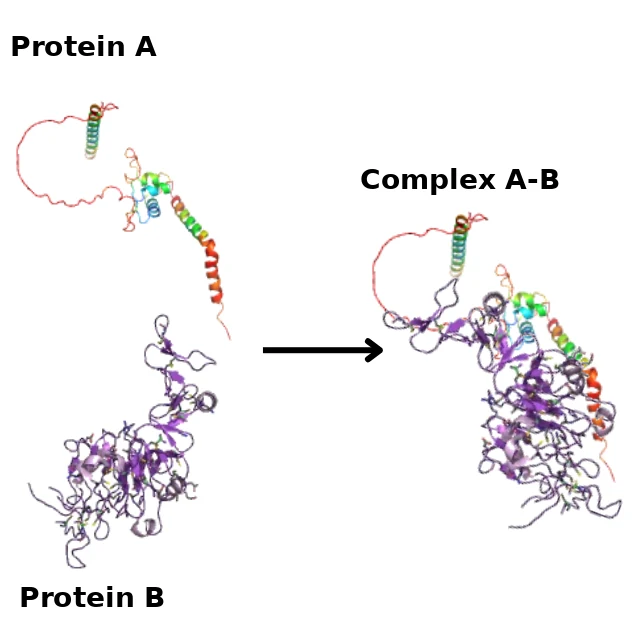
\includegraphics[width=0.8\linewidth]{fig_2_2}
      \caption{Duas proteínas formando um complexo.}
    \end{figure}
  \end{columns}
\end{frame}

\begin{frame}{Descrição do Problema}
  \begin{block}{Problema}
    Atribuir a cada proteína seus termos da \textit{Gene Ontology} em BP, CC e MF, a partir da sua sequência de aminoácidos e
    da sua vizinhança na rede STRING.
  \end{block}
  \vspace{0.6em}
  \begin{itemize}\setlength{\itemsep}{0.5em}
    \item Cerca de 500 termos por ontologia, respeitando a hierarquia
    \item Uma única rede agregada e multiespécie, com evidências heterogêneas
    \item Cerca de um terço das proteínas não tem nenhuma interação mantida, e um modelo só de rede não vê nada
      nelas
  \end{itemize}
\end{frame}

\begin{frame}{Objetivos}
  \begin{block}{Objetivo geral}
    Desenvolver, avaliar e combinar abordagens baseadas em redes PPI para a anotação funcional multirrótulo,
    integrando a topologia da rede a \textit{embeddings} da sequência de aminoácidos.
  \end{block}
\end{frame}

\begin{frame}{Questões de Pesquisa (1/2)}
  \begin{itemize}\setlength{\itemsep}{0.7em}
    \item<+-> \textbf{(QP1)} Como diferentes representações dos dados da rede PPI do STRING afetam a qualidade da predição de função nos três domínios da GO?
    \item<+-> \textbf{(QP2)} Em que medida a propagação fixa dos \textit{embeddings} do ProtT5 pela rede STRING melhora a representação só de rede, e como esse efeito varia entre BP, MF e CC?
    \item<+-> \textbf{(QP3)} Como se comparam estratégias que vão de \textit{embeddings} de grafo simples à propagação fixa não paramétrica e às GNNs, sob um protocolo experimental comum e com cabeças de classificação vetorial e visual?
    \item<+-> \textbf{(QP4)} As fusões precoce e tardia melhoram a métrica principal em relação aos seus componentes de propagação fixa e de GNN?
  \end{itemize}
\end{frame}

\begin{frame}{Questões de Pesquisa (2/2)}
  \begin{itemize}\setlength{\itemsep}{0.7em}
    \item<+-> \textbf{(QP5)} Como a profundidade da propagação e o coeficiente de retenção afetam o desempenho, e a partir de que ponto propagar mais começa a diluir o sinal da própria proteína?
    \item<+-> \textbf{(QP6)} Como a abordagem proposta se compara a algoritmos de referência baseados em rede, com todos os métodos avaliados nas mesmas partições e no mesmo cenário transdutivo?
    \item<+-> \textbf{(QP7)} A metodologia funciona aplicada diretamente a redes globais de evidências agregadas (várias fontes de interação e várias espécies numa única topologia), sem particionar o grafo por espécie ou por canal de evidência?
  \end{itemize}
\end{frame}

% =================================================================================== Background
\section{Fundamentação Teórica}

\begin{frame}{Grafos, Adjacência e Passagem de Mensagens}
  \begin{columns}[c]
    \column{0.44\textwidth}
    \begin{itemize}\setlength{\itemsep}{0.4em}
      \item $G=(V,E,w)$: proteínas, associações, confiança do STRING
      \item Matriz de adjacência $A$; armazenamento esparso em $O(|E|)$
      \item Passagem de mensagens: agregar os vizinhos e depois atualizar o nó
      \item $L$ camadas alcançam $L$ saltos; camadas demais causam \textit{oversmoothing}
    \end{itemize}
    \column{0.54\textwidth}
    \begin{figure}
      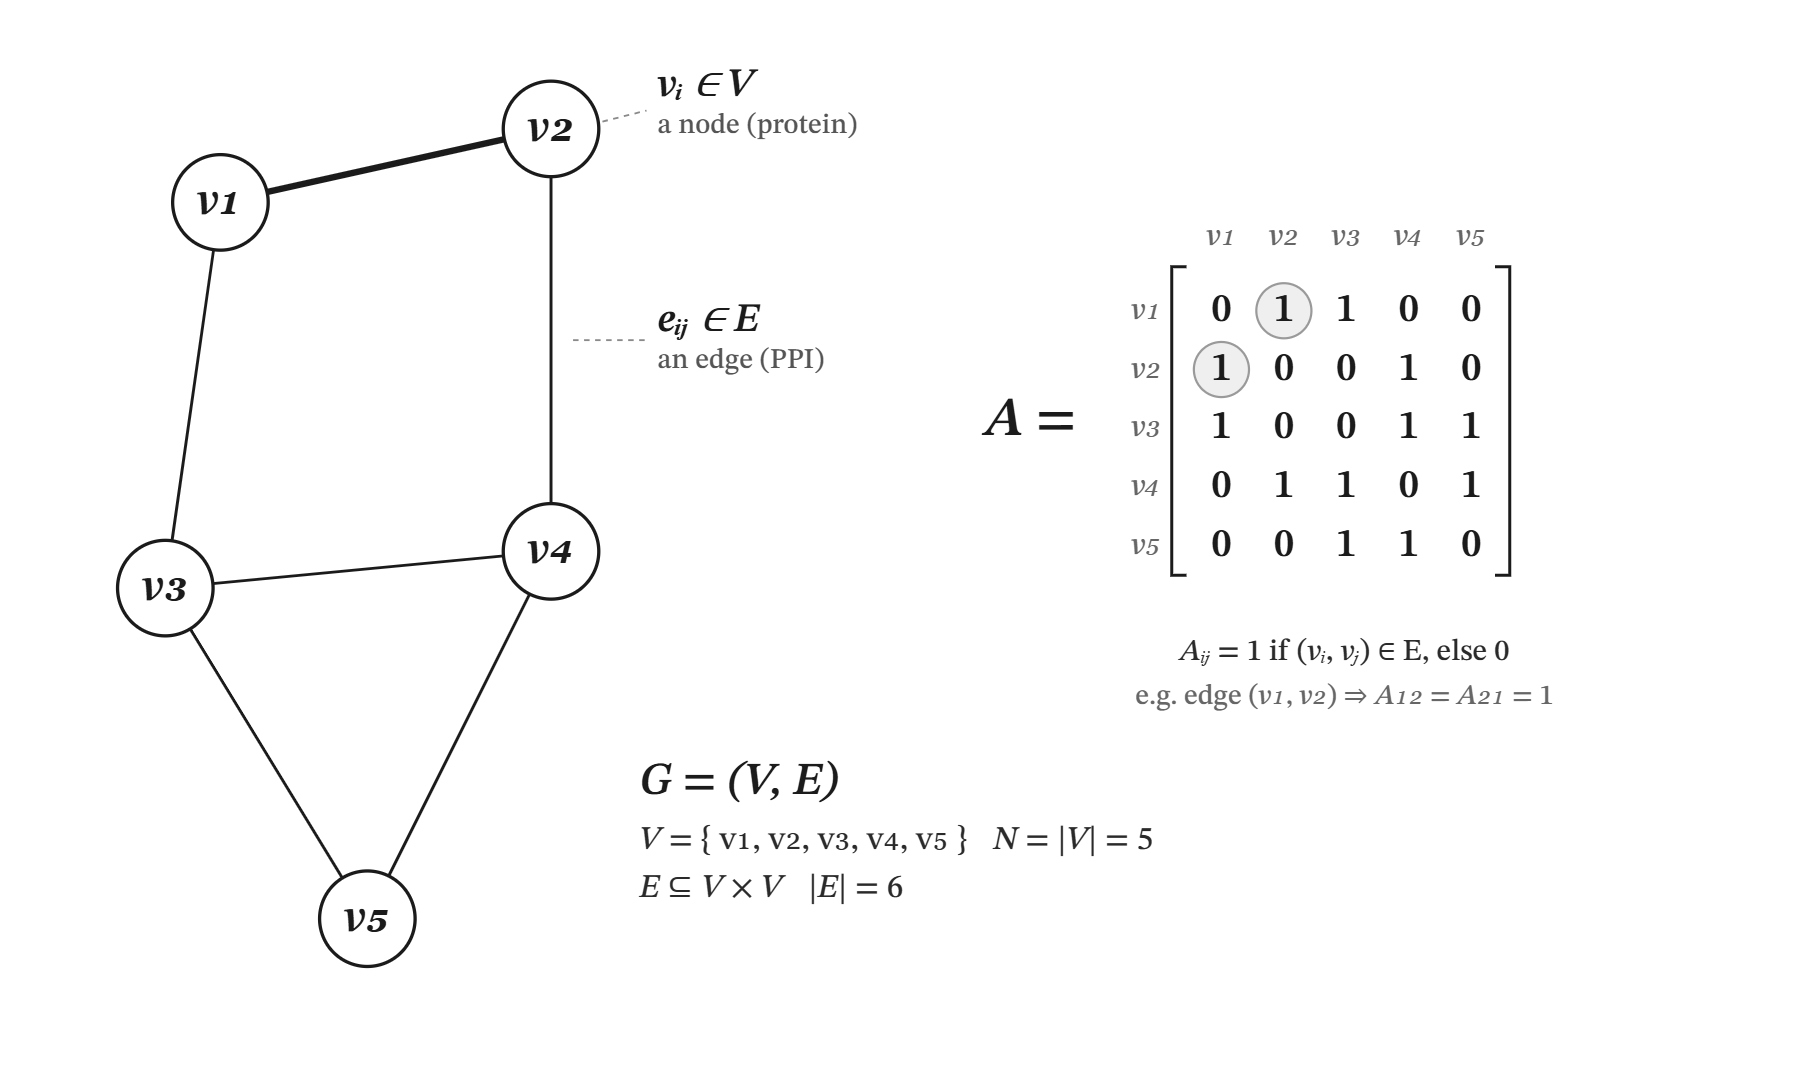
\includegraphics[width=\linewidth]{fig_2_3}
      \caption{Notação de grafos e matriz de adjacência.}
    \end{figure}
  \end{columns}
\end{frame}

\begin{frame}{Redes Neurais em Grafos: GCN e GAT}
  \begin{columns}[c]
    \column{0.47\textwidth}
    \begin{itemize}\setlength{\itemsep}{0.45em}
      \item \textbf{GCN}~\cite{kipf2017semi}: normalização simétrica de $W+I$, seguida de uma transformação aprendida
      \item \textbf{GAT}~\cite{velickovic2018graph}: pesos de atenção aprendidos sobre os vizinhos
      \item \textbf{Configuração neste trabalho:} 2 camadas de largura 1.024; na GAT, 4 cabeças de atenção e o escore da aresta como atributo
      \item Os operadores aprendidos rodam no grafo inteiro a cada passo de treinamento
    \end{itemize}
    \column{0.51\textwidth}
    \begin{eqbox}[\linewidth]
      $\displaystyle \mathbf{H}^{(\ell+1)}=\phi\Big(\tilde{D}^{-1/2}\,\tilde{W}\,\tilde{D}^{-1/2}\,\mathbf{H}^{(\ell)}\,\Theta^{(\ell)}\Big)$
      \\[0.9em]
      $\displaystyle a_{ij}=\frac{\exp(e_{ij})}{\sum_{k\in\mathcal{N}(i)\cup\{i\}}\exp(e_{ik})}$
    \end{eqbox}
    {\scriptsize $\tilde{W}=W+I$ e $\tilde{D}$ é sua matriz de graus; $e_{ij}$ pontua o par $(i,j)$ a partir das duas
    extremidades e da aresta.}
  \end{columns}
\end{frame}

\begin{frame}{Modelos de Linguagem de Proteínas}
  \begin{itemize}\setlength{\itemsep}{0.5em}
    \item Pré-treinamento autossupervisionado em coleções muito grandes de sequências de proteínas
    \item Codificador \textit{transformer}: cada resíduo é lido no contexto de todos os outros
    \item \textbf{ProtT5-XL-U50}~\cite{elnaggar2021prottrans}: codificador T5 treinado no BFD e depois no UniRef50, com
      15\% dos resíduos mascarados
    \item Usado aqui como extrator congelado de características
    \item Toda proteína tem um \textit{embedding} de sequência, com ou sem arestas na rede
  \end{itemize}
\end{frame}

% =================================================================================== Related work
\section{Trabalhos Correlatos}

\begin{frame}{Da Votação entre Vizinhos aos \textit{Transformers} em Grafos}
  \begin{center}
  \begin{tikzpicture}[node distance=0.25cm, box/.style={draw=navy, rounded corners=2pt, align=center, font=\small,
      minimum height=0.9cm, text width=2.15cm, fill=blockbody}]
    \node[box] (a) {votação entre\\vizinhos};
    \node[box, right=of a] (b) {difusão};
    \node[box, right=of b] (c) {\textit{embeddings}\\de nós};
    \node[box, right=of c] (d) {híbridos\\e GNNs};
    \node[box, right=of d] (e) {\textit{transformers}\\em grafos};
    \foreach \x/\y in {a/b,b/c,c/d,d/e} \draw[-{Latex}, navy] (\x) -- (\y);
  \end{tikzpicture}
  \end{center}
  \vspace{0.3em}
  \begin{itemize}\setlength{\itemsep}{0.4em}
    \item Cada etapa acrescentou parâmetros, ajustes e custo
    \item Métodos só de rede não conseguem pontuar uma proteína ausente da rede
    \item Métodos recentes alcançam proteínas fora da rede por busca de homologia
  \end{itemize}
\end{frame}

\begin{frame}{Cinco Métodos Reimplementados neste Trabalho}
  \begin{table}\footnotesize
    \caption{Onde cada método guarda seus parâmetros aprendidos e como trata as proteínas fora da rede.}
    \begin{tabular}{@{}lp{6.6cm}l@{}}\toprule
      Método & Parâmetros aprendidos & Proteínas fora da rede \\ \midrule
      Mashup~\cite{cho2016compact} & nenhum na difusão, todos na compressão & não pontuadas \\
      deepNF~\cite{deepnf} & nenhum na difusão, todos na compressão & não pontuadas \\
      MELISSA~\cite{wu2024melissa} & rótulos injetados na construção da rede & não pontuadas \\
      DeepGraphGO~\cite{you_deepgraphgo_2021} & entre os passos de propagação & busca de homologia \\
      SEGT-GO~\cite{wang2025segtgo} & após uma agregação não paramétrica de múltiplos saltos, num \textit{transformer} & busca de homologia \\
      \bottomrule
    \end{tabular}
  \end{table}
  \vspace{0.2em}
  Os cinco foram retreinados no mesmo corpus, nas mesmas partições e no mesmo grafo transdutivo.
\end{frame}

\begin{frame}{Lacuna de Pesquisa}
  \begin{alertblock}{Questão em aberto}
    \centering Um componente de grafo aprendido ainda é necessário quando o objeto propagado já é informativo?
  \end{alertblock}
  \vspace{0.5em}
  \begin{itemize}\setlength{\itemsep}{0.45em}
    \item \textbf{Proposta:} propagar \textit{embeddings} do ProtT5 com um operador fixo de passos finitos e usar uma cabeça comum
    \item Toda proteína tem uma representação de sequência, então a rede complementa em vez de ser a única fonte
    \item Nenhuma rota visual anterior parte de um \textit{embedding} propagado de modelo de linguagem
  \end{itemize}
\end{frame}

% =================================================================================== Materials and methods
\section{Materiais e Métodos}

\begin{frame}{Base de Dados: Corpus Derivado do CAFA5}
  \begin{table}\small
    \caption{Proteínas por partição e termos mantidos por ontologia.}
    \TabCorpus
  \end{table}
  \begin{itemize}\setlength{\itemsep}{0.3em}
    \item Dados de treinamento do CAFA5, consolidados em trabalho anterior do grupo~\cite{oliveira2025supermagov2}
    \item Partição 80\,/\,10\,/\,10, disjunta por proteína, sem restrição temporal ou de homologia
    \item Rótulos por proteína (média): 25,91 em BP, 12,48 em CC e 7,55 em MF
    \item Densidade da matriz de rótulos: 5,18\%, 2,51\% e 1,51\%
  \end{itemize}
\end{frame}

\begin{frame}{STRING v11.5: Uma Única Rede Agregada}
  \begin{columns}[c]
    \column{0.42\textwidth}
    \begin{itemize}\setlength{\itemsep}{0.4em}\small
      \item 2.422.234 registros, 791.011 pares distintos, 86.423 proteínas
      \item Escore combinado em $[0{,}400;\ 0{,}999]$: confiança, não força de ligação
      \item Cada par se repete 3,06 vezes em média (até 170), sempre com o mesmo escore
      \item \textbf{Graus:} cauda pesada, mediana de 5 a 7, máximo entre 763 e 805
    \end{itemize}
    \column{0.56\textwidth}
    \begin{figure}
      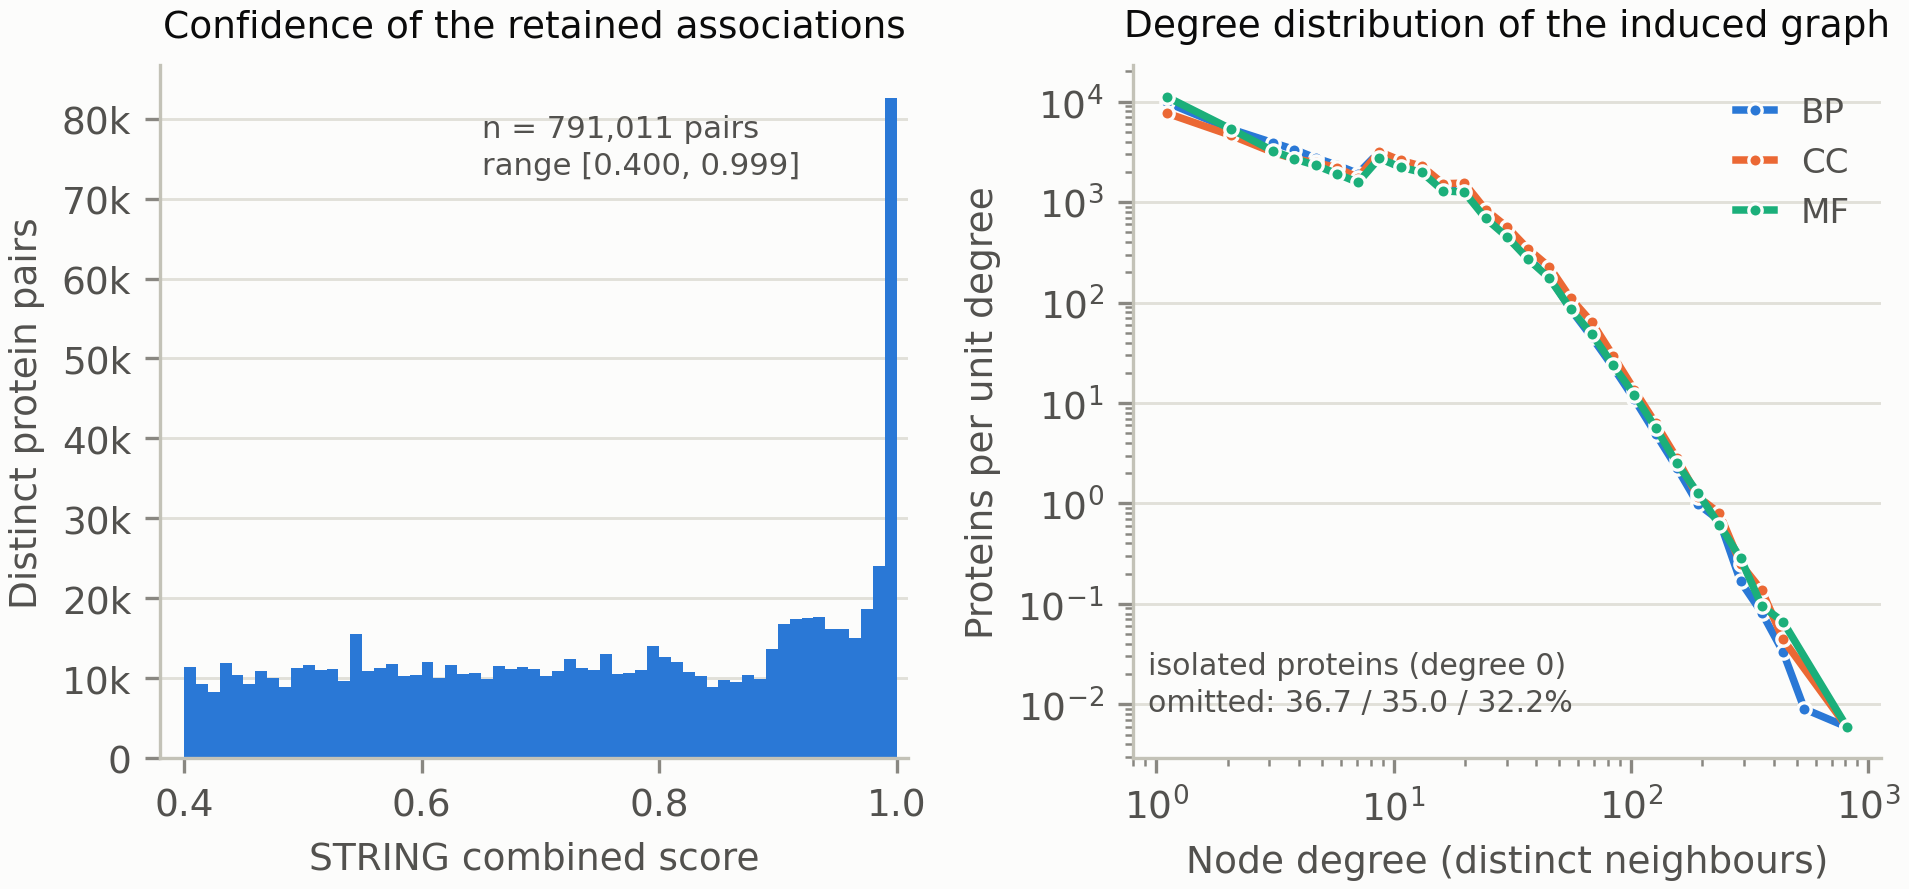
\includegraphics[width=\linewidth]{fig_4_1}
      \caption{Escore dos pares mantidos e distribuição de graus.}
    \end{figure}
  \end{columns}
\end{frame}

\begin{frame}{Um Terço das Proteínas Não Tem Arestas}
  \begin{itemize}
    \item \textbf{Isoladas:} 36,65\% em BP, 34,95\% em CC e 32,19\% em MF, estáveis entre treinamento, validação e teste
    \item Limiares até 0,40 não têm efeito; em 0,90, mais da metade das proteínas fica isolada
  \end{itemize}
  \begin{columns}[c]
    \column{0.49\textwidth}
    \begin{figure}
      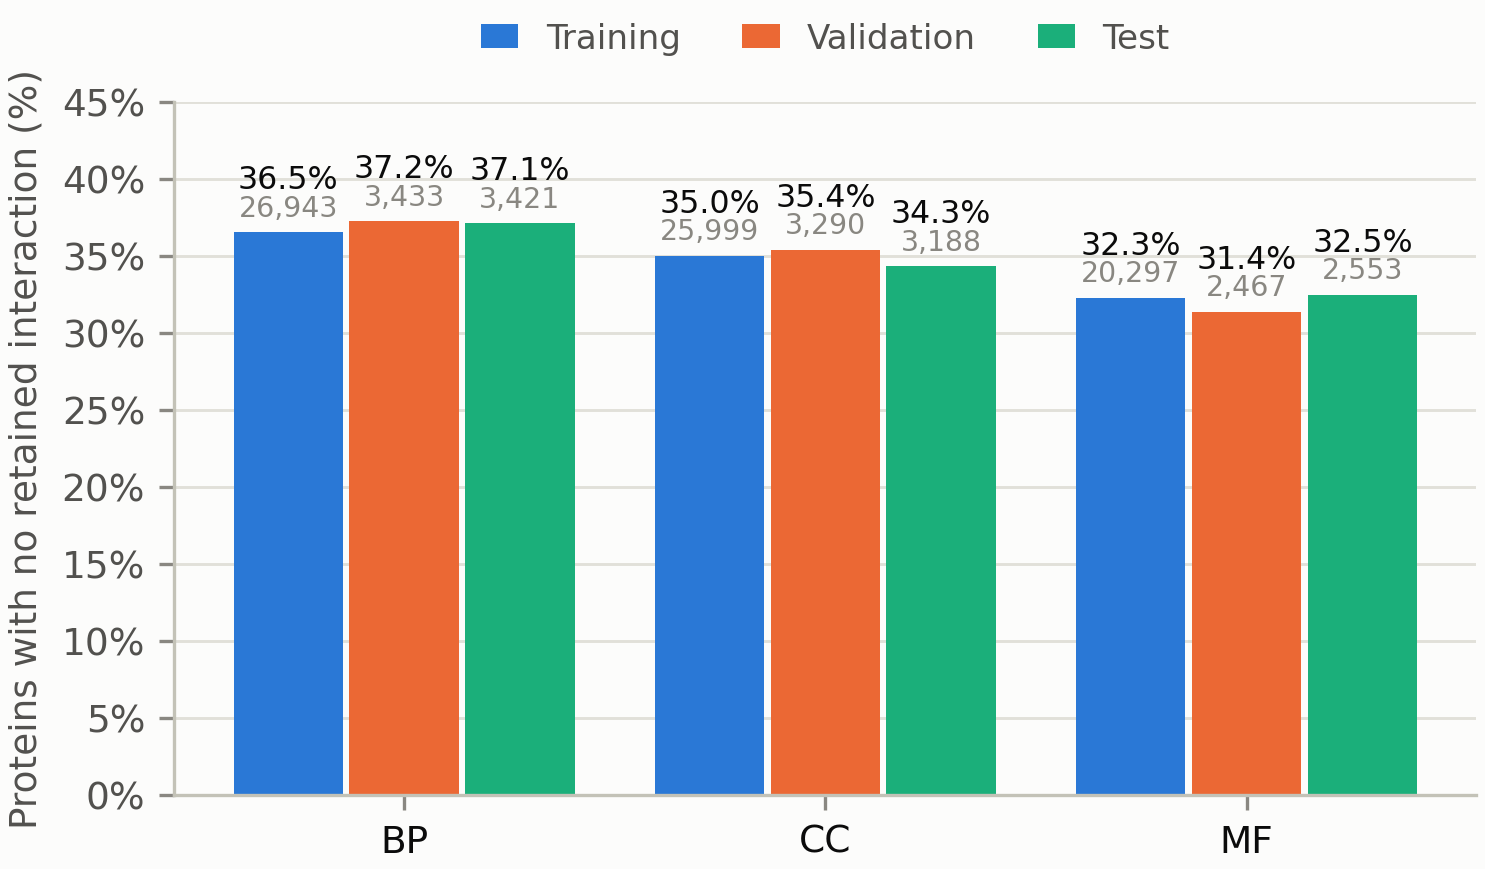
\includegraphics[width=0.9\linewidth]{fig_4_2}
      \caption{Proteínas isoladas por partição.}
    \end{figure}
    \column{0.49\textwidth}
    \begin{figure}
      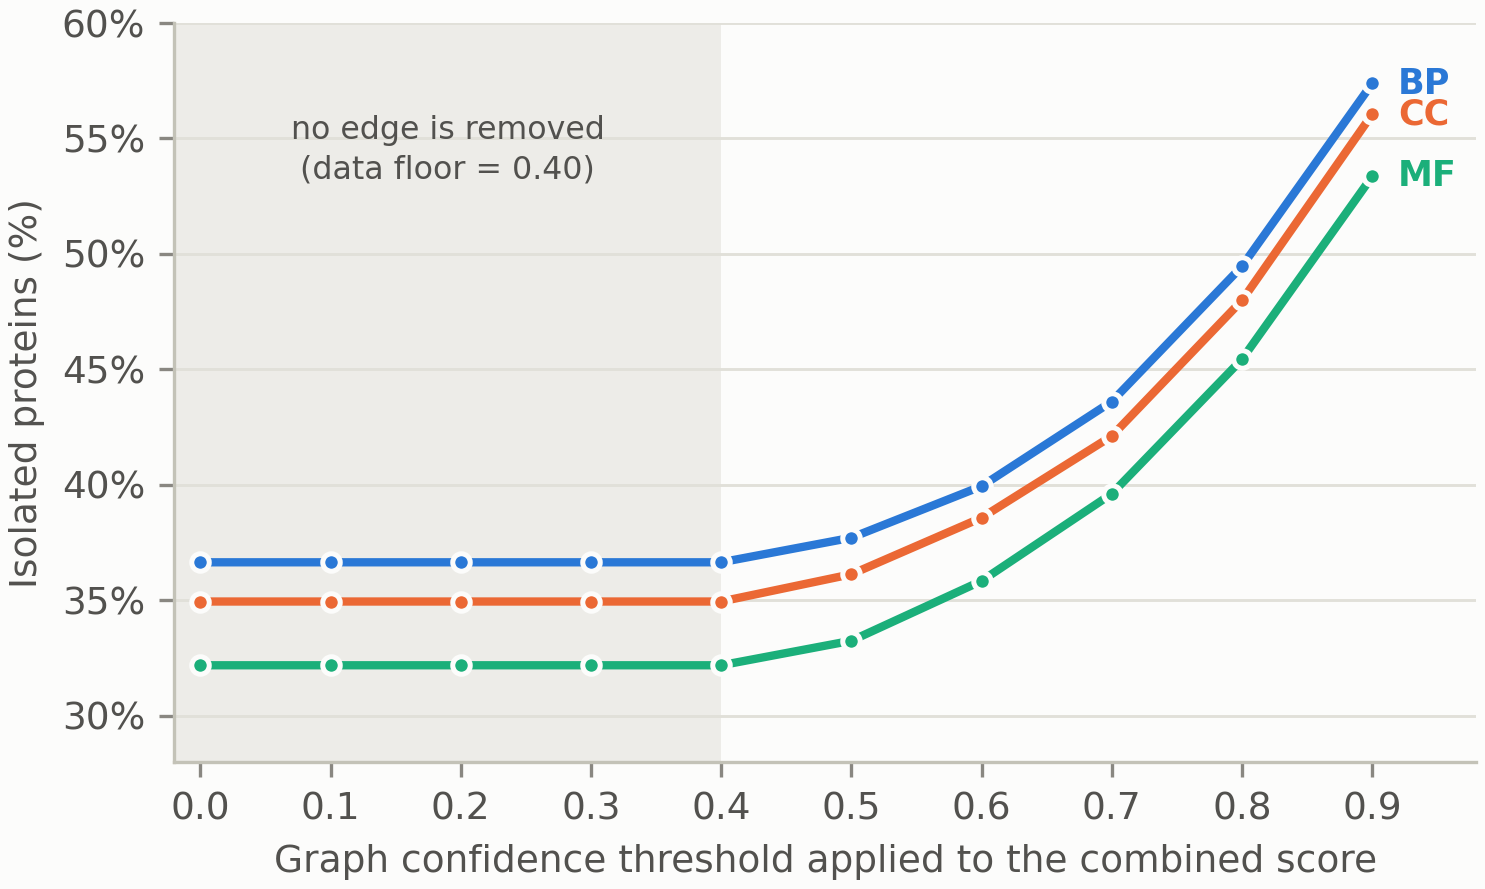
\includegraphics[width=0.9\linewidth]{fig_4_3}
      \caption{Proteínas isoladas por limiar de escore.}
    \end{figure}
  \end{columns}
\end{frame}

\begin{frame}{Métricas de Avaliação}
  \textbf{Critério principal:} $\wF$, a medida $F$ ponderada pelo conteúdo de informação (IC)
  \begin{eqbox}[0.86\textwidth]
    $\displaystyle \wF=\max_{\tau}\frac{2\,\mathrm{wpr}(\tau)\,\mathrm{wrc}(\tau)}{\mathrm{wpr}(\tau)+\mathrm{wrc}(\tau)},
    \qquad \mathrm{IC}(v)=-\log_2 P\big(v\mid \mathrm{pa}(v)\big)$
  \end{eqbox}
  \begin{itemize}\setlength{\itemsep}{0.35em}
    \item Também $F_{\max}$, $F^{*}_{\max}$, $\Smin$, AuPRC e IAuPRC
    \item Predições tornadas consistentes com a hierarquia antes da avaliação
    \item 101 limiares; modo de avaliação completo: proteína sem predição conta como revocação zero
  \end{itemize}
\end{frame}

\begin{frame}{Protocolo Experimental}
  \begin{figure}
    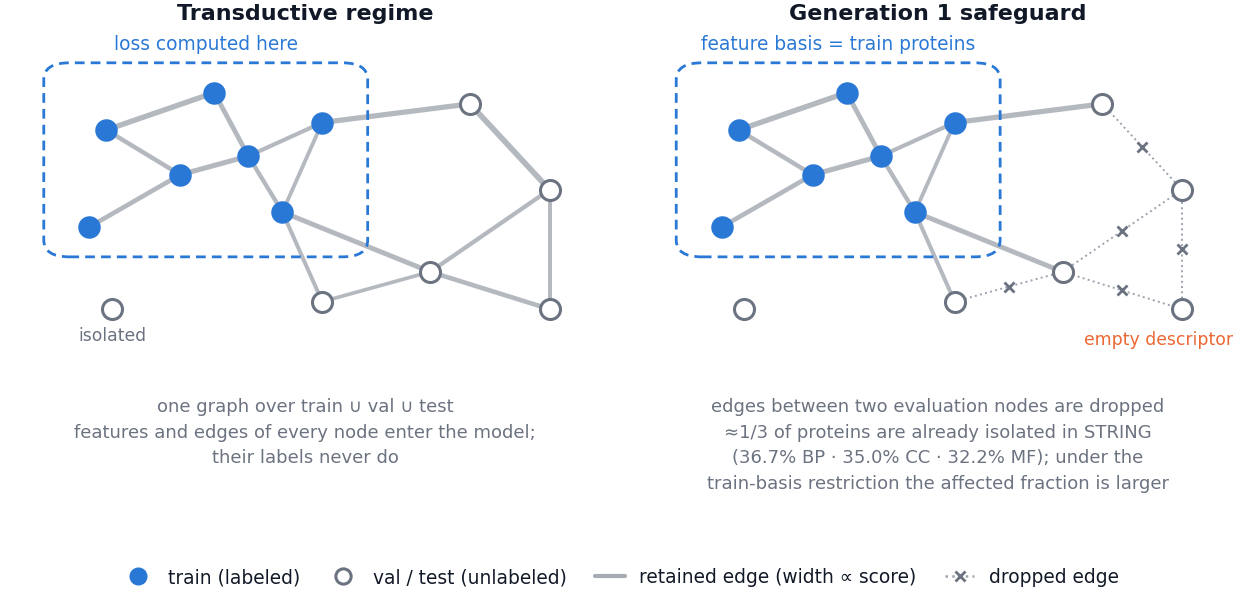
\includegraphics[height=0.46\textheight]{fig_5_2}
    \caption{Regime transdutivo: um grafo sobre todas as proteínas, com rótulos lidos só nas de treinamento.}
  \end{figure}
  \begin{itemize}\setlength{\itemsep}{0.3em}
    \item Toda decisão de projeto tomada na validação; o teste lido uma única vez, no fim
    \item \textbf{Semente única:} diferenças abaixo de 0,5\,p.p. são lidas como empates
  \end{itemize}
\end{frame}

\begin{frame}{Metodologia: Duas Gerações, Três Decisões}
  \begin{columns}[c]
    \column{0.34\textwidth}
    \begin{itemize}\setlength{\itemsep}{0.45em}
      \item \textbf{Todo modelo:} representação, propagação, cabeça de predição
      \item \textbf{Geração 1:} apenas a rede
        \begin{itemize}
          \item Cerca de um terço isolado: descritor nulo
        \end{itemize}
      \item \textbf{Geração 2 (NEXUS-GO):} ProtT5 mais a rede
    \end{itemize}
    \column{0.64\textwidth}
    \begin{figure}
      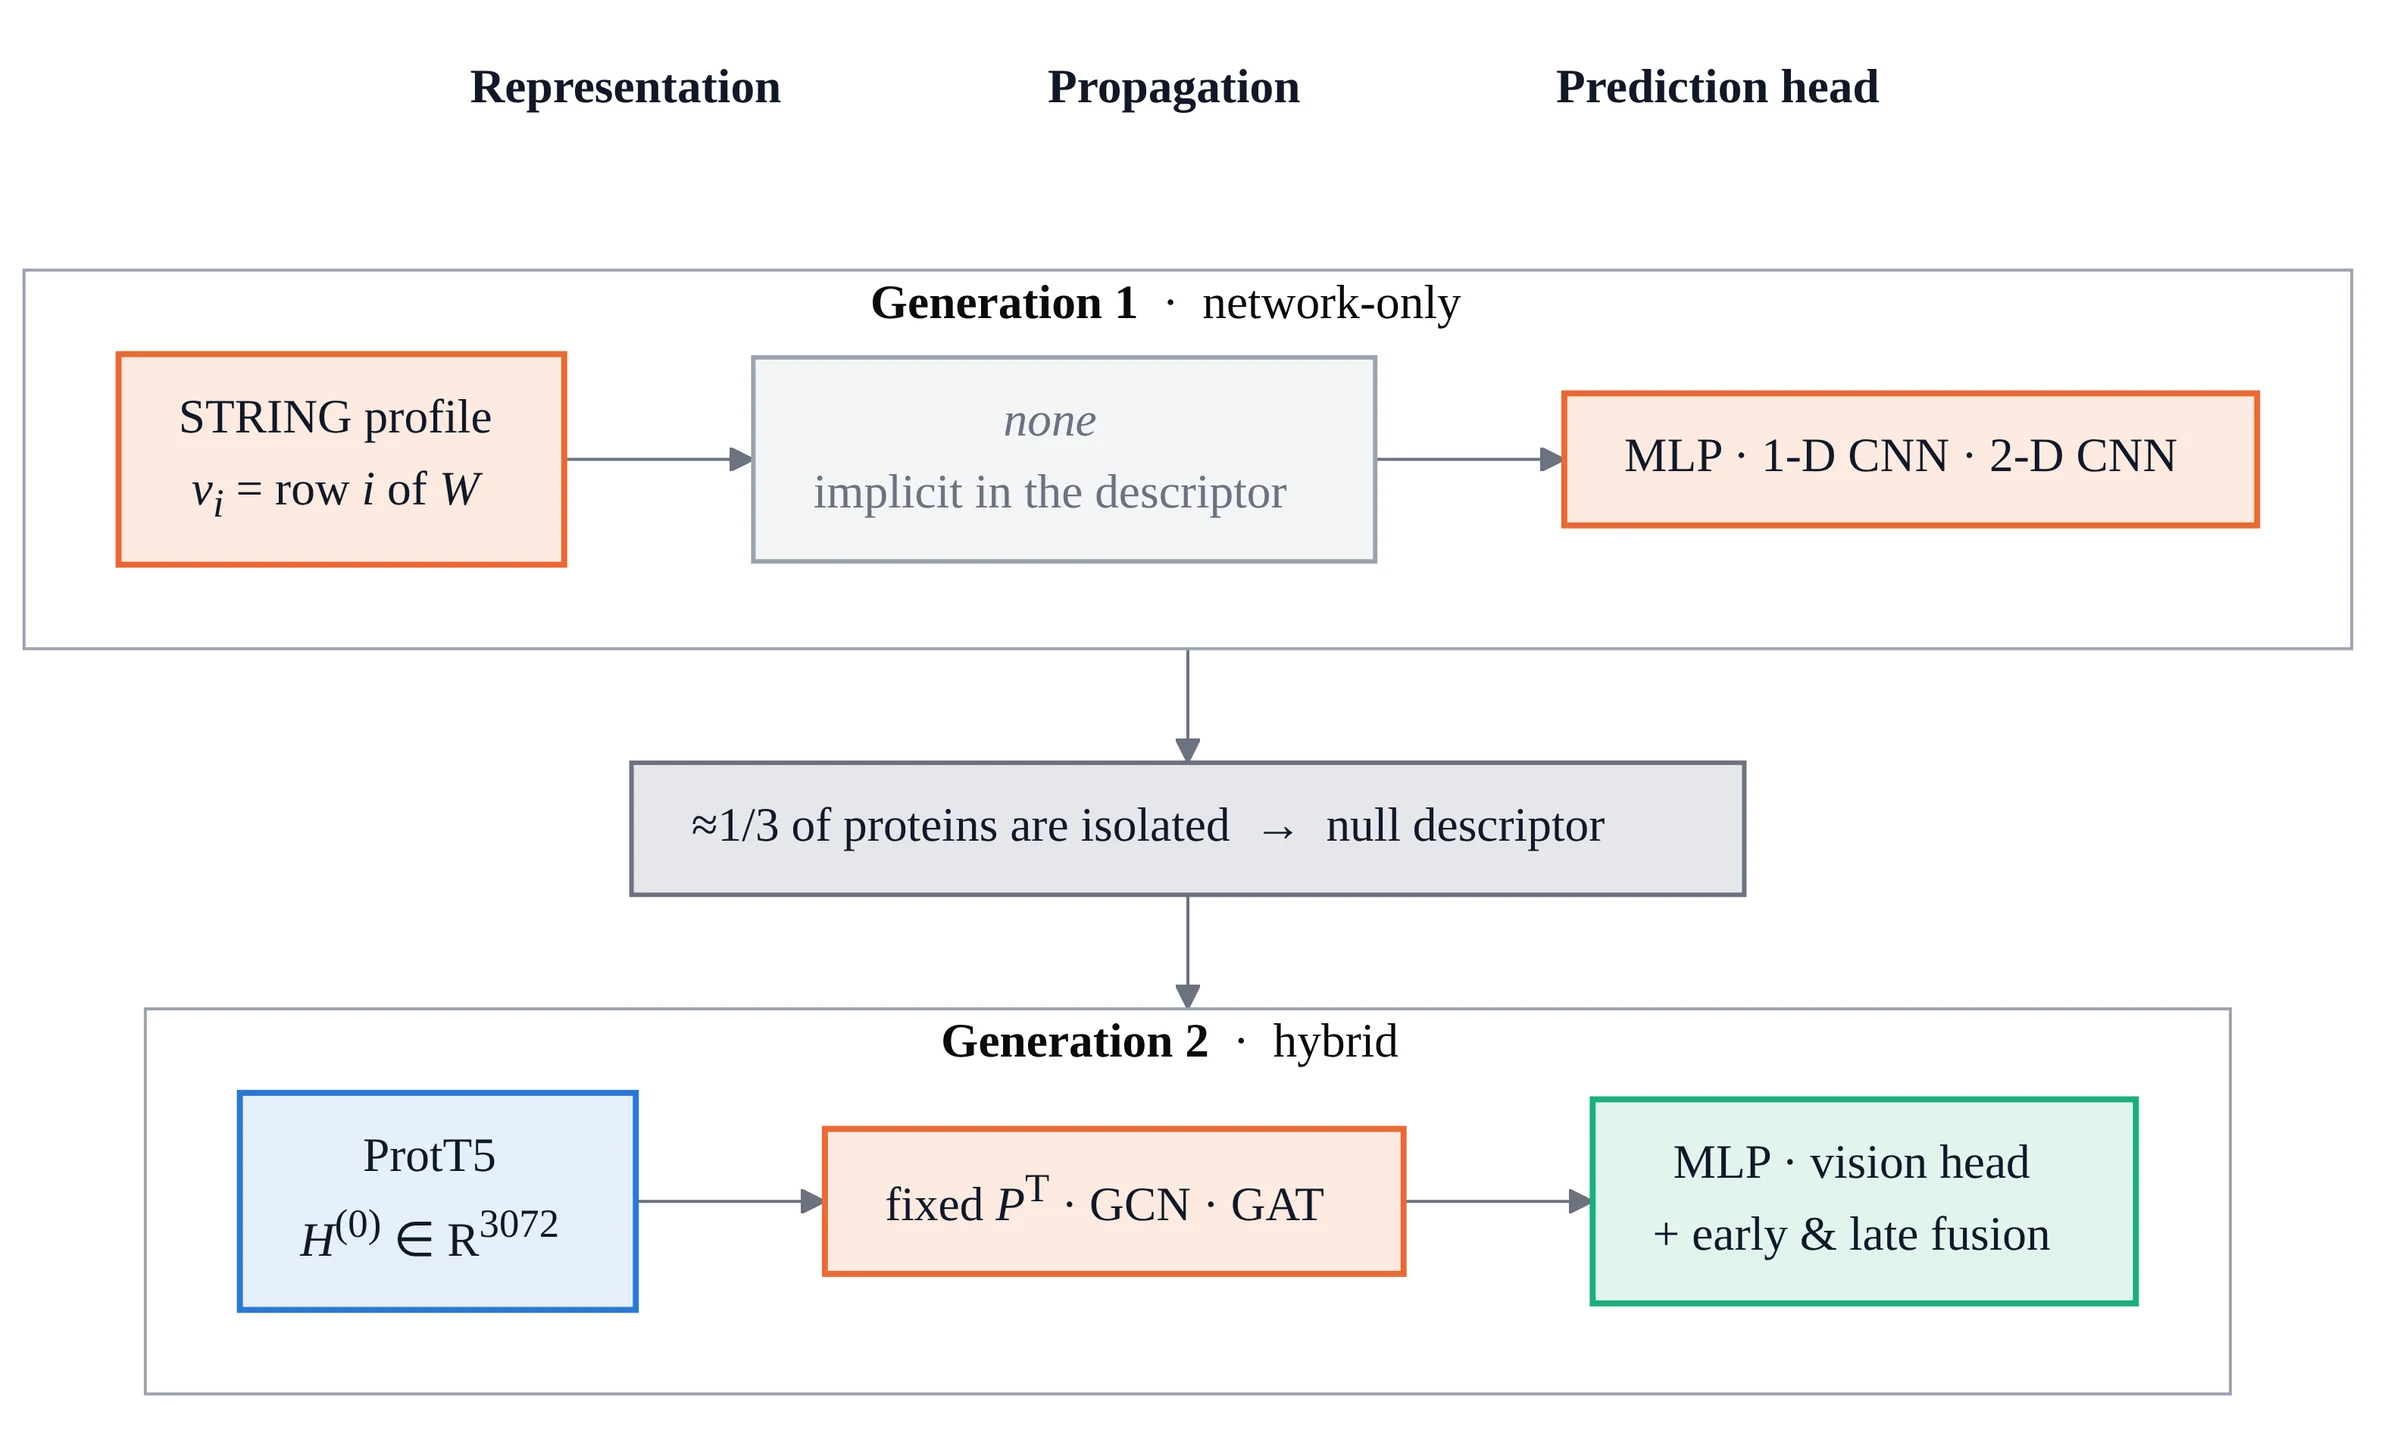
\includegraphics[width=\linewidth]{fig_5_1}
      \caption{As duas gerações ao longo das três decisões.}
    \end{figure}
  \end{columns}
\end{frame}

\begin{frame}{Geração 1: Apenas a Rede}
  \begin{columns}[c]
    \column{0.18\textwidth}
    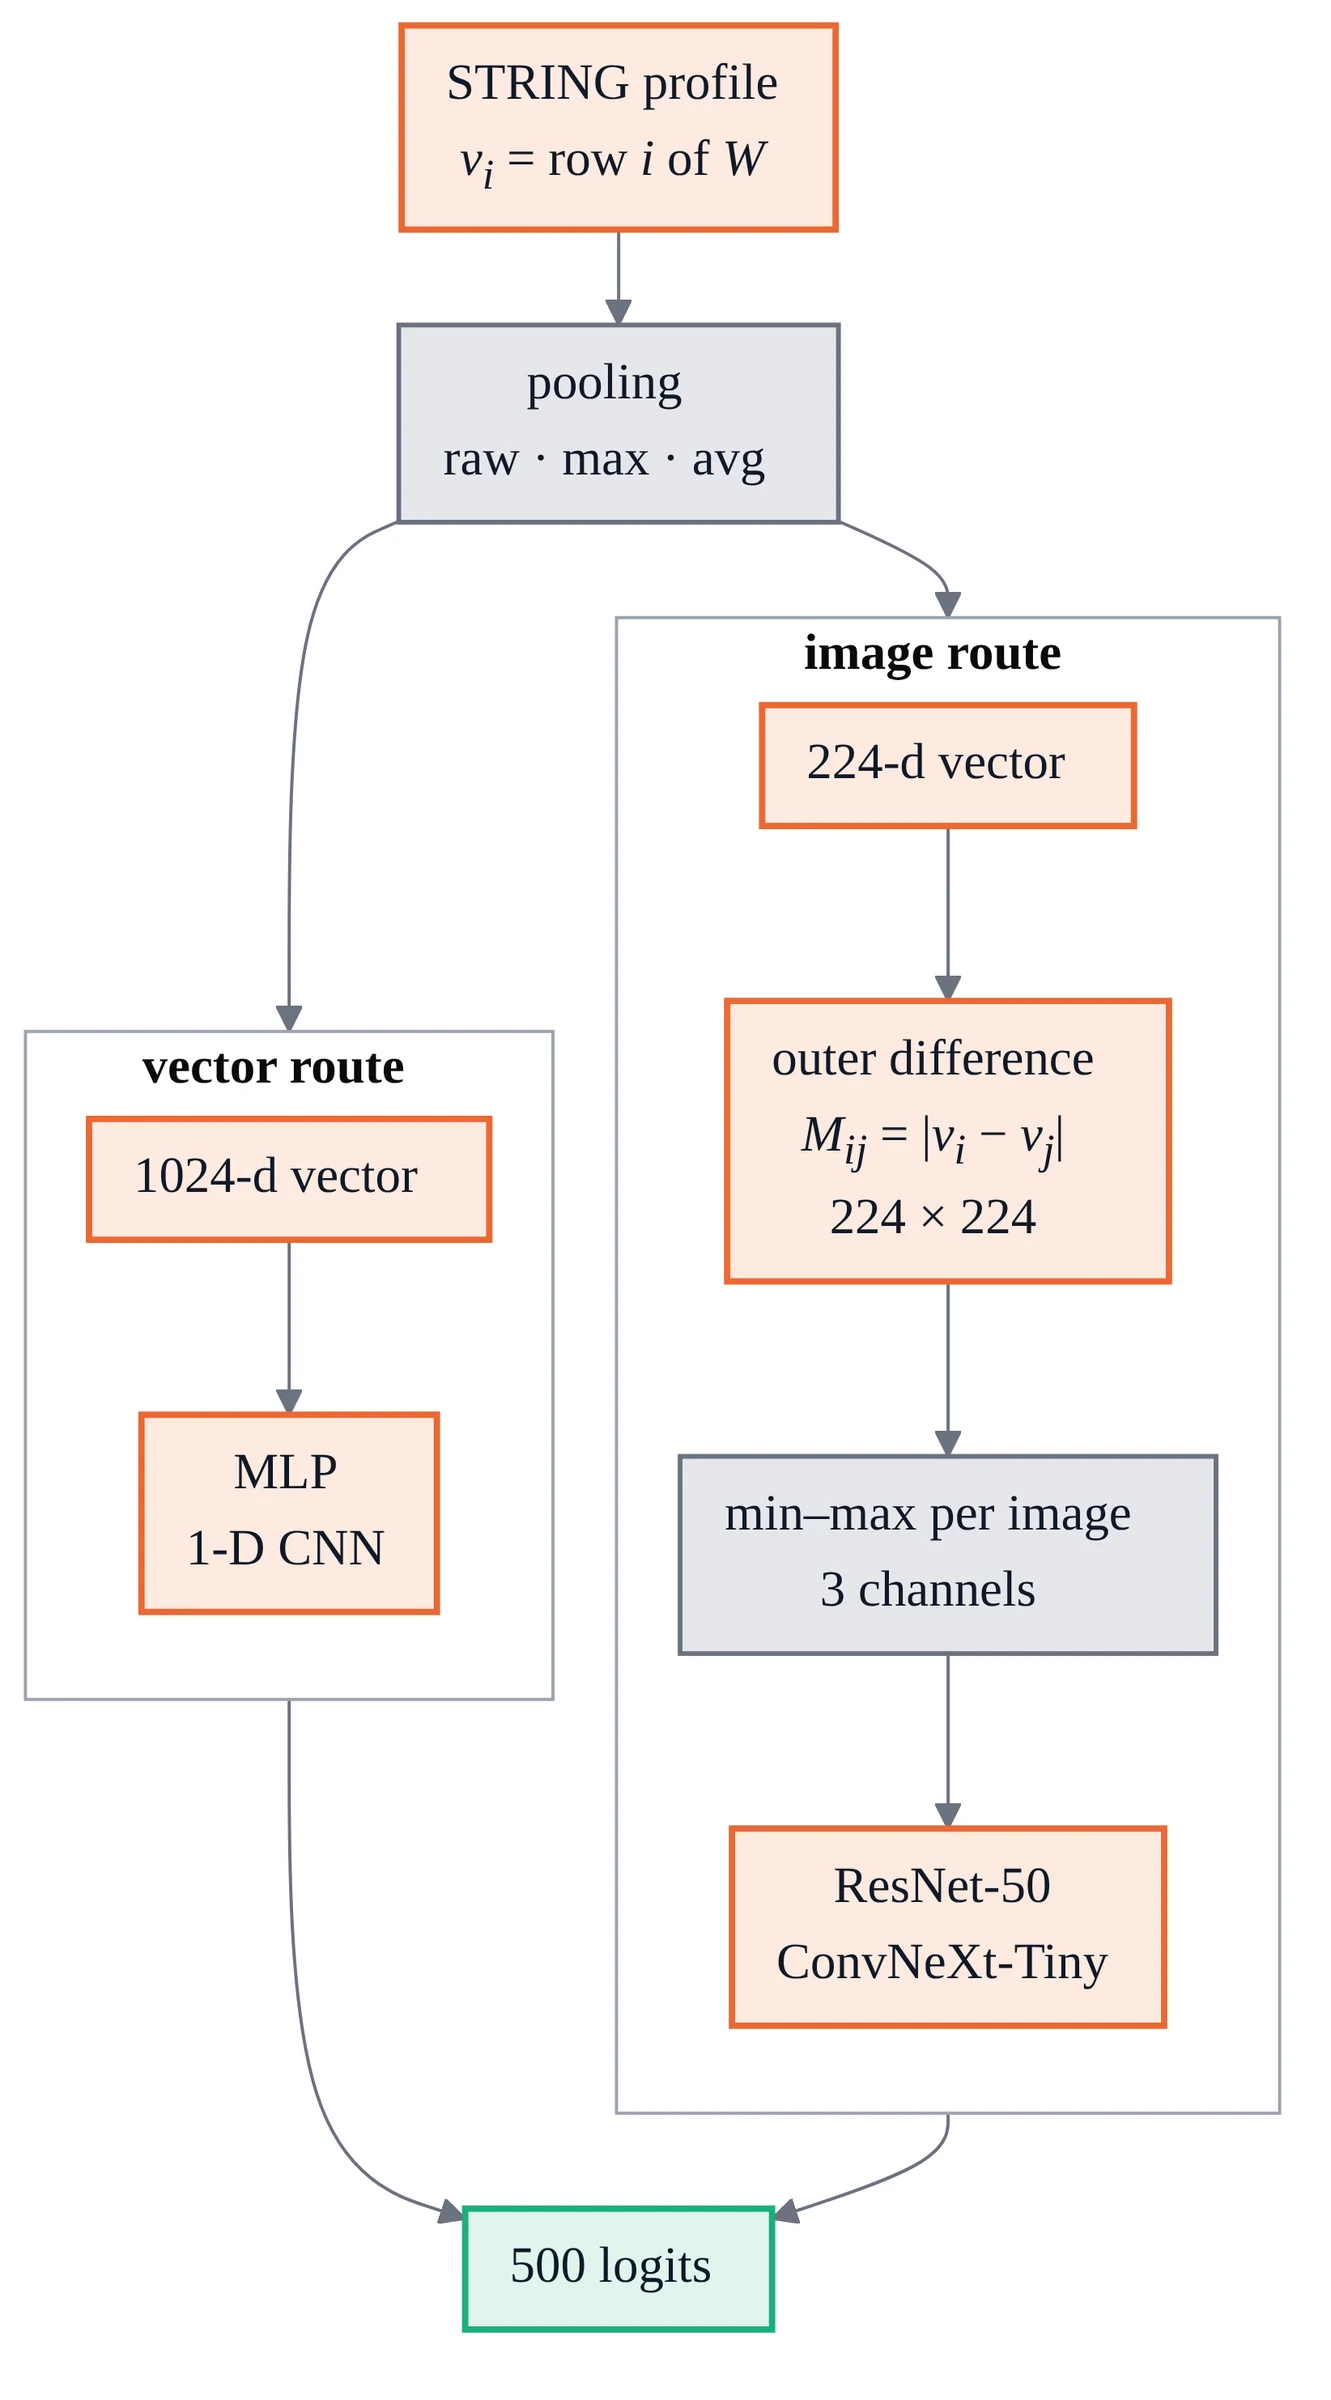
\includegraphics[width=\linewidth, height=0.72\textheight, keepaspectratio]{fig_5_3}
    \column{0.8\textwidth}
    \begin{itemize}\setlength{\itemsep}{0.2em}\small
      \item \textbf{Entrada:} a linha da proteína na adjacência ponderada, restrita às proteínas de treinamento
      \item \textbf{\textit{Pooling}:} \textit{raw}, \textit{max} ou \textit{avg}
      \item \textbf{Rota vetorial:} MLP ou CNN 1-D
      \item \textbf{Rota visual:} matriz de diferenças $224\times224$, ResNet-50 ou ConvNeXt-Tiny
      \item \textbf{Piso:} um \textit{baseline} ingênuo de frequência de termos
    \end{itemize}
    \begin{figure}
      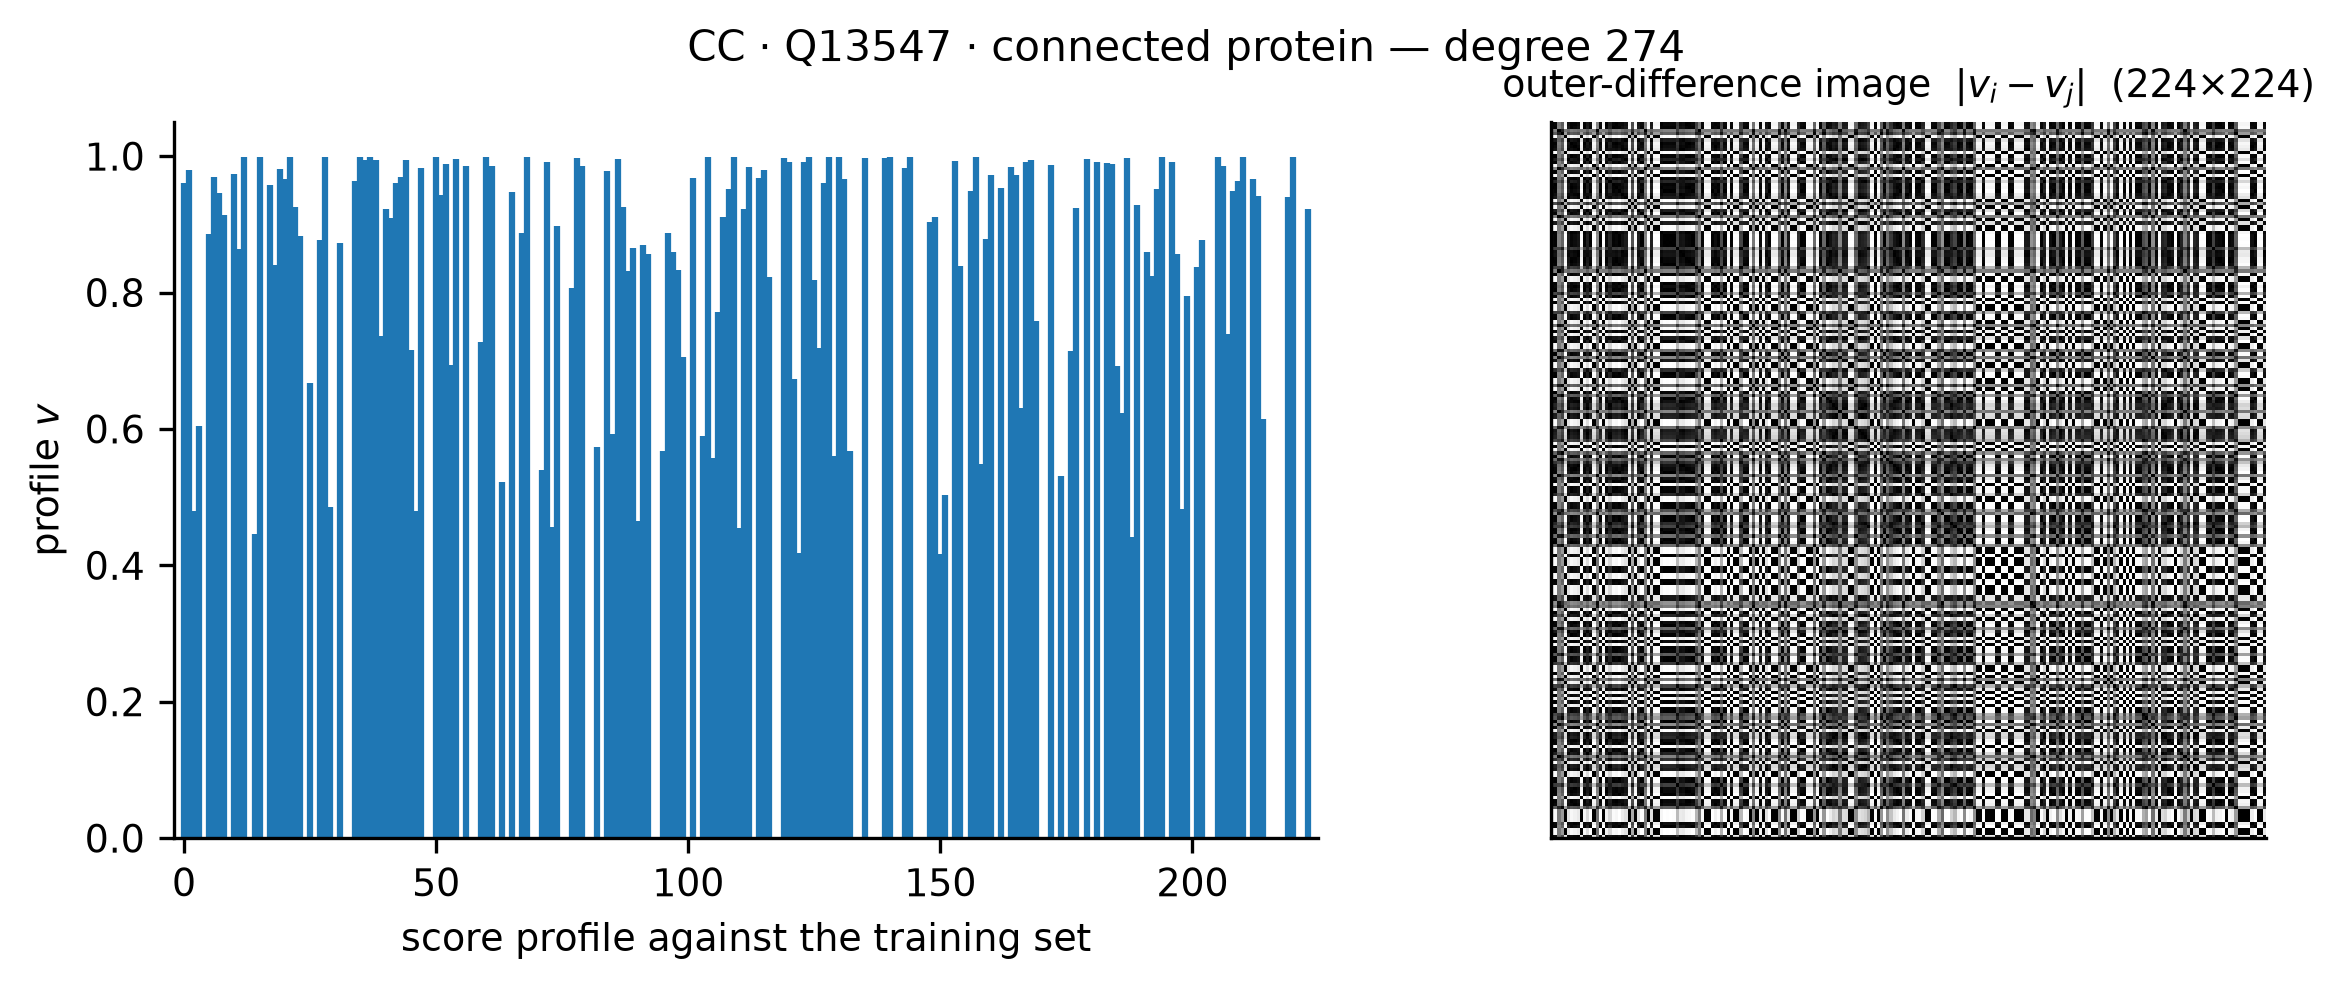
\includegraphics[height=0.32\textheight]{fig_5_4}
      \caption{Uma proteína conectada: seu perfil e sua imagem de diferenças externas.}
    \end{figure}
  \end{columns}
\end{frame}

\begin{frame}{Uma Proteína Isolada Não Tem Entrada}
  \begin{figure}
    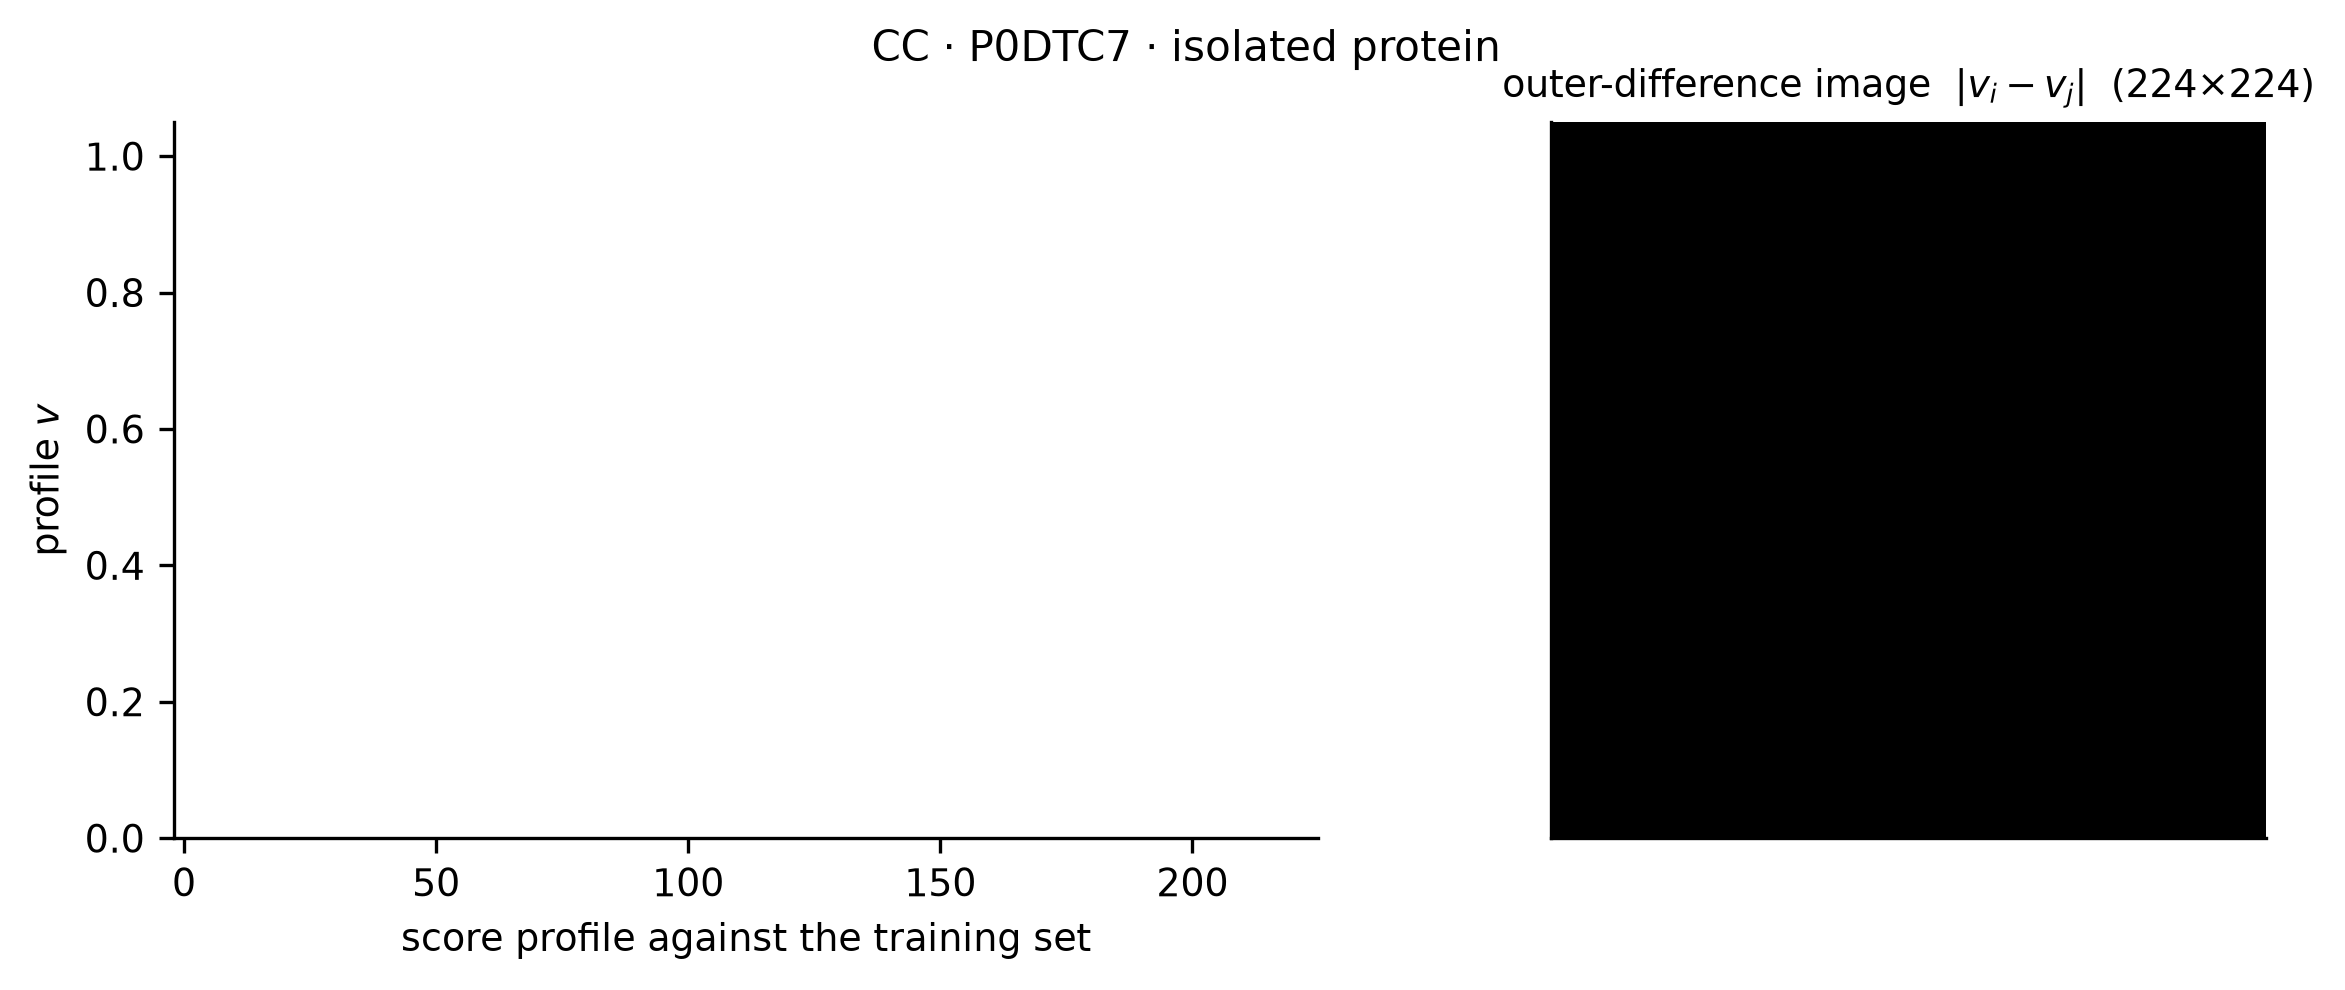
\includegraphics[height=0.42\textheight]{fig_5_5}
    \caption{Uma proteína isolada: perfil nulo e imagem uniforme.}
  \end{figure}
  \begin{itemize}\setlength{\itemsep}{0.3em}
    \item Perfil e matriz nulos, imagem uniforme: a cabeça só devolve a frequência das classes
    \item Nenhuma arquitetura recupera o que está ausente
    \item \textbf{Requisito:} uma representação que exista para toda proteína
  \end{itemize}
\end{frame}

\begin{frame}{Geração 2: NEXUS-GO}
  \begin{center}
  \begin{tikzpicture}[font=\small, >={Latex},
      b/.style={draw, rounded corners=2pt, align=center, minimum height=0.8cm, inner sep=4pt},
      r/.style={b, draw=navy, fill=blockbody, text width=2.9cm}]
    \node[b, draw=seq, text=seq] (seq) at (0,1.2) {Sequência};
    \node[b, draw=seq, text=seq, right=0.6cm of seq] (pt5) {ProtT5\\$H^{(0)}\in\mathbb{R}^{3072}$};
    \node[b, draw=net, text=net] (str) at (0,-1.2) {STRING};
    \node[b, draw=net, text=net, right=0.6cm of str] (w) {grafo $W$\\$P=W D_c^{-1}$};
    \draw[->, seq] (seq) -- (pt5); \draw[->, net] (str) -- (w);
    \node[r, right=1.4cm of pt5, yshift=-0.2cm] (fix) {\NX{Fixed}\\propagação fixa};
    \node[r, right=1.4cm of w, yshift=0.2cm] (gnn) {\NX{GNN}\\aprendida (GCN, GAT)};
    \draw[->] (pt5) -- (fix); \draw[->] (w) -- (fix.west);
    \draw[->] (pt5) -- (gnn.west); \draw[->] (w) -- (gnn);
    \node[r, draw=fus, fill=fus!8, right=1.2cm of fix, yshift=-0.85cm] (early) {\NX{Early}\\une as\\representações};
    \node[r, draw=fus, fill=fus!8, below=0.25cm of early] (late) {\NX{Late}\\combina as\\probabilidades};
    \draw[->, fus] (fix.east) -- (early.west); \draw[->, fus] (gnn.east) -- (early.west);
    \draw[->, fus] (fix.east) -- (late.west); \draw[->, fus] (gnn.east) -- (late.west);
    \only<2>{\node[hl, fit=(seq)(pt5)(str)(w)] {};}
    \only<3>{\node[hl, fit=(fix)] {};}
    \only<4>{\node[hl, fit=(gnn)] {};}
    \only<5>{\node[hl, fit=(early)(late)] {};}
  \end{tikzpicture}
  \end{center}
  \vspace{0.4em}
  \begin{overprint}
    \onslide<1>\centering Duas entradas e quatro rotas; a Geração 1 fica como controle só de topologia.
    \onslide<2>\centering O ProtT5 existe para toda proteína; o STRING dá o grafo ponderado $W$ e o operador $P$.
    \onslide<3>\centering \NX{Fixed}: propagação sem parâmetros, calculada uma vez e guardada em \textit{cache}.
    \onslide<4>\centering \NX{GNN}: GCN ou GAT, recalculada a cada passo de treinamento.
    \onslide<5>\centering \NX{Early} une as duas representações; \NX{Late} combina as suas probabilidades.
  \end{overprint}
\end{frame}

\begin{frame}{ProtT5-XL-U50 Congelado: Três Camadas}
  \begin{figure}
    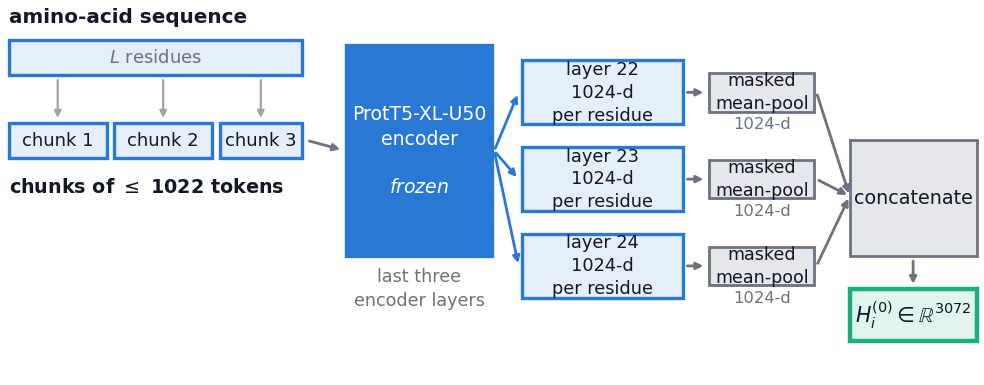
\includegraphics[width=0.66\linewidth]{fig_5_7}
    \caption{Extração da representação do ProtT5.}
  \end{figure}
  \begin{itemize}\setlength{\itemsep}{0.3em}
    \item Trechos de até 1.022 resíduos; média mascarada por trecho e entre os trechos
    \item Camadas 24, 23 e 22, concatenadas: $3\times1{.}024=3{.}072$ dimensões
    \item Existe para toda proteína, isolada ou não
  \end{itemize}
\end{frame}

\begin{frame}{Propagação Fixa: Sem Parâmetros}
  \begin{eqbox}[0.84\textwidth]
    $\displaystyle H^{(h)} = \alpha\,H^{(h-1)} + (1-\alpha)\,P^{\top}H^{(h-1)},\qquad h=1,\dots,T$
    \\[0.7em]
    $\displaystyle H^{(T)} = \sum_{k=0}^{T}\binom{T}{k}\,\alpha^{T-k}(1-\alpha)^{k}\,\big(P^{\top}\big)^{k}H^{(0)}$
  \end{eqbox}
  \begin{itemize}\setlength{\itemsep}{0.3em}\small
    \item $P = W D_c^{-1}$ é estocástica por coluna: os pesos são relativos aos vizinhos de cada proteína
    \item Duplicatas do STRING fundidas com max, que preserva o escore (a soma o multiplicaria)
    \item Calculada uma vez, em \textit{cache}, reutilizada a cada época; $T=0$ ou $\alpha=1$ desliga o grafo
    \item Ao contrário do PageRank personalizado, o estado inicial nunca é reintroduzido
  \end{itemize}
\end{frame}

\begin{frame}{Propagação em Quatro Proteínas Reais}
  \begin{columns}[c]
    \column{0.56\textwidth}
    \begin{figure}
      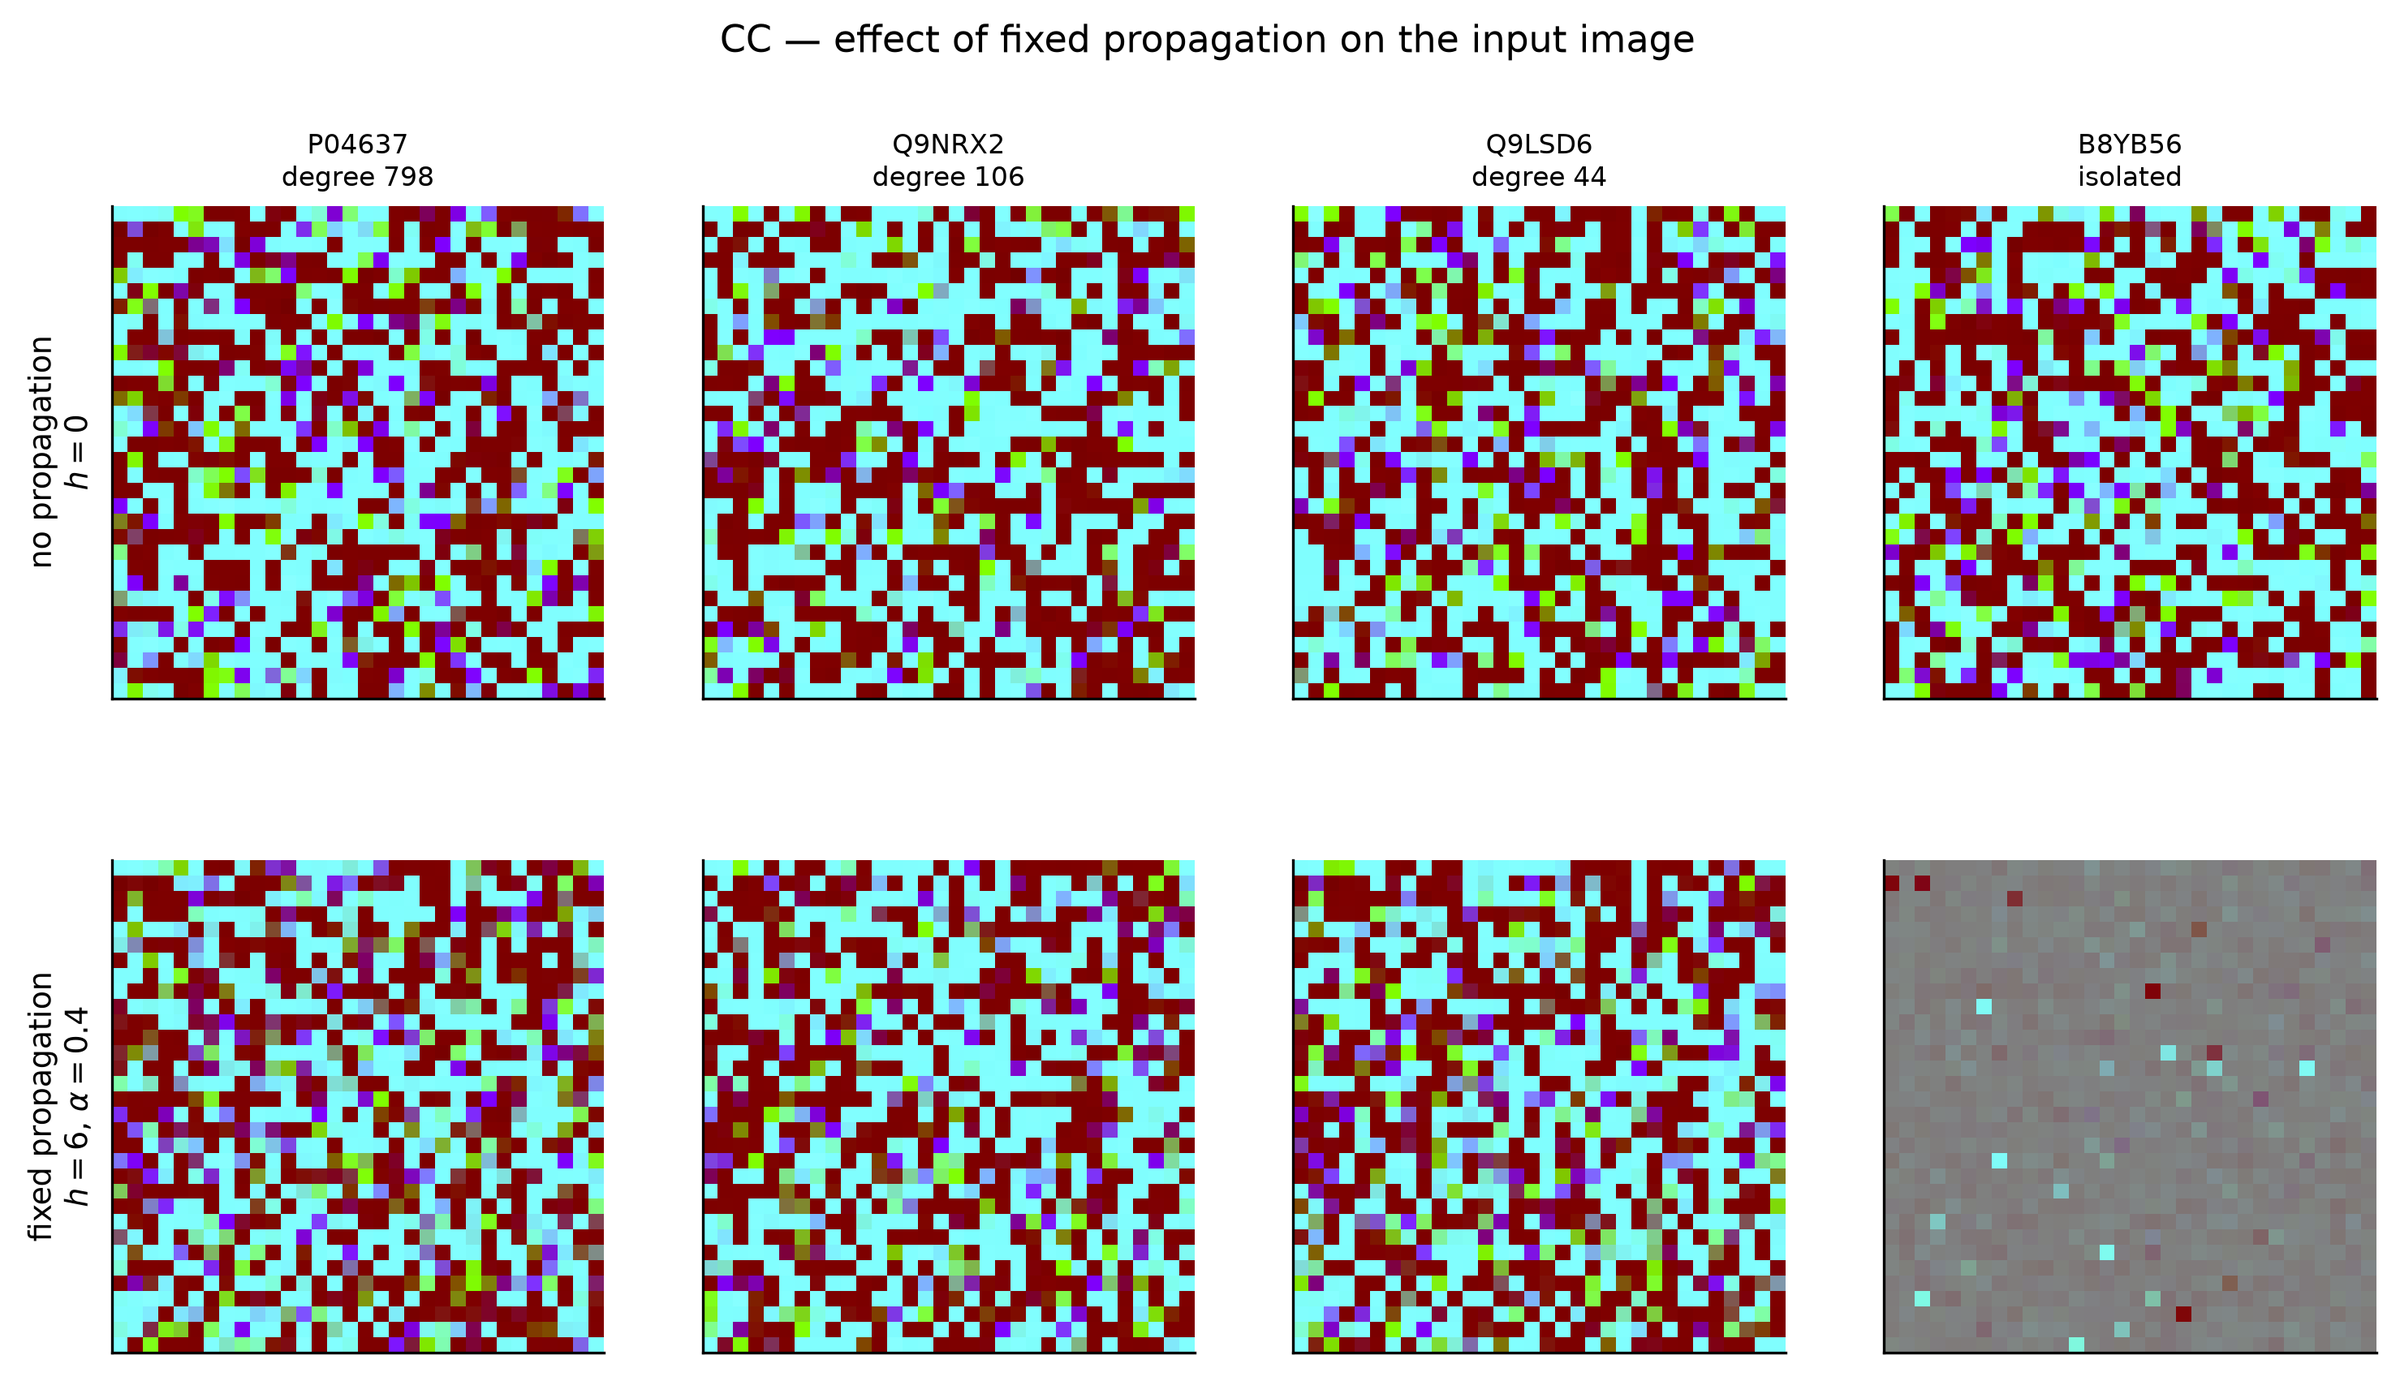
\includegraphics[width=\linewidth]{fig_5_8}
      \caption{Imagens CC de quatro proteínas: $T=0$ (acima) e $T=6$, $\alpha=0{,}4$ (abaixo).}
    \end{figure}
    \column{0.42\textwidth}
    \begin{itemize}\setlength{\itemsep}{0.45em}
      \item Proteínas conectadas mantêm sua estrutura e absorvem a vizinhança
      \item Uma proteína isolada vira $\alpha^{T}H^{(0)}$: mesma direção, escala menor
      \item Logo, seus ganhos não podem vir de informação da vizinhança
    \end{itemize}
  \end{columns}
\end{frame}

\begin{frame}{Cabeças de Predição: Vetorial e Visual}
  \begin{itemize}\setlength{\itemsep}{0.25em}
    \item \textbf{Vetorial:} MLP com camadas de 1.024 e 512, normalização em lote, \textit{dropout} de 0,4
    \item \textbf{Visual:} $\sigma(\mathrm{clip}(z))$ dividido em três canais $32\times32$, um por camada do ProtT5
    \item \textbf{\textit{Backbones}:} ResNet-50~\cite{he2016deep} e ConvNeXt-Tiny~\cite{liu2022convnet} (ImageNet), com ajuste fino
      completo
  \end{itemize}
  \begin{figure}
    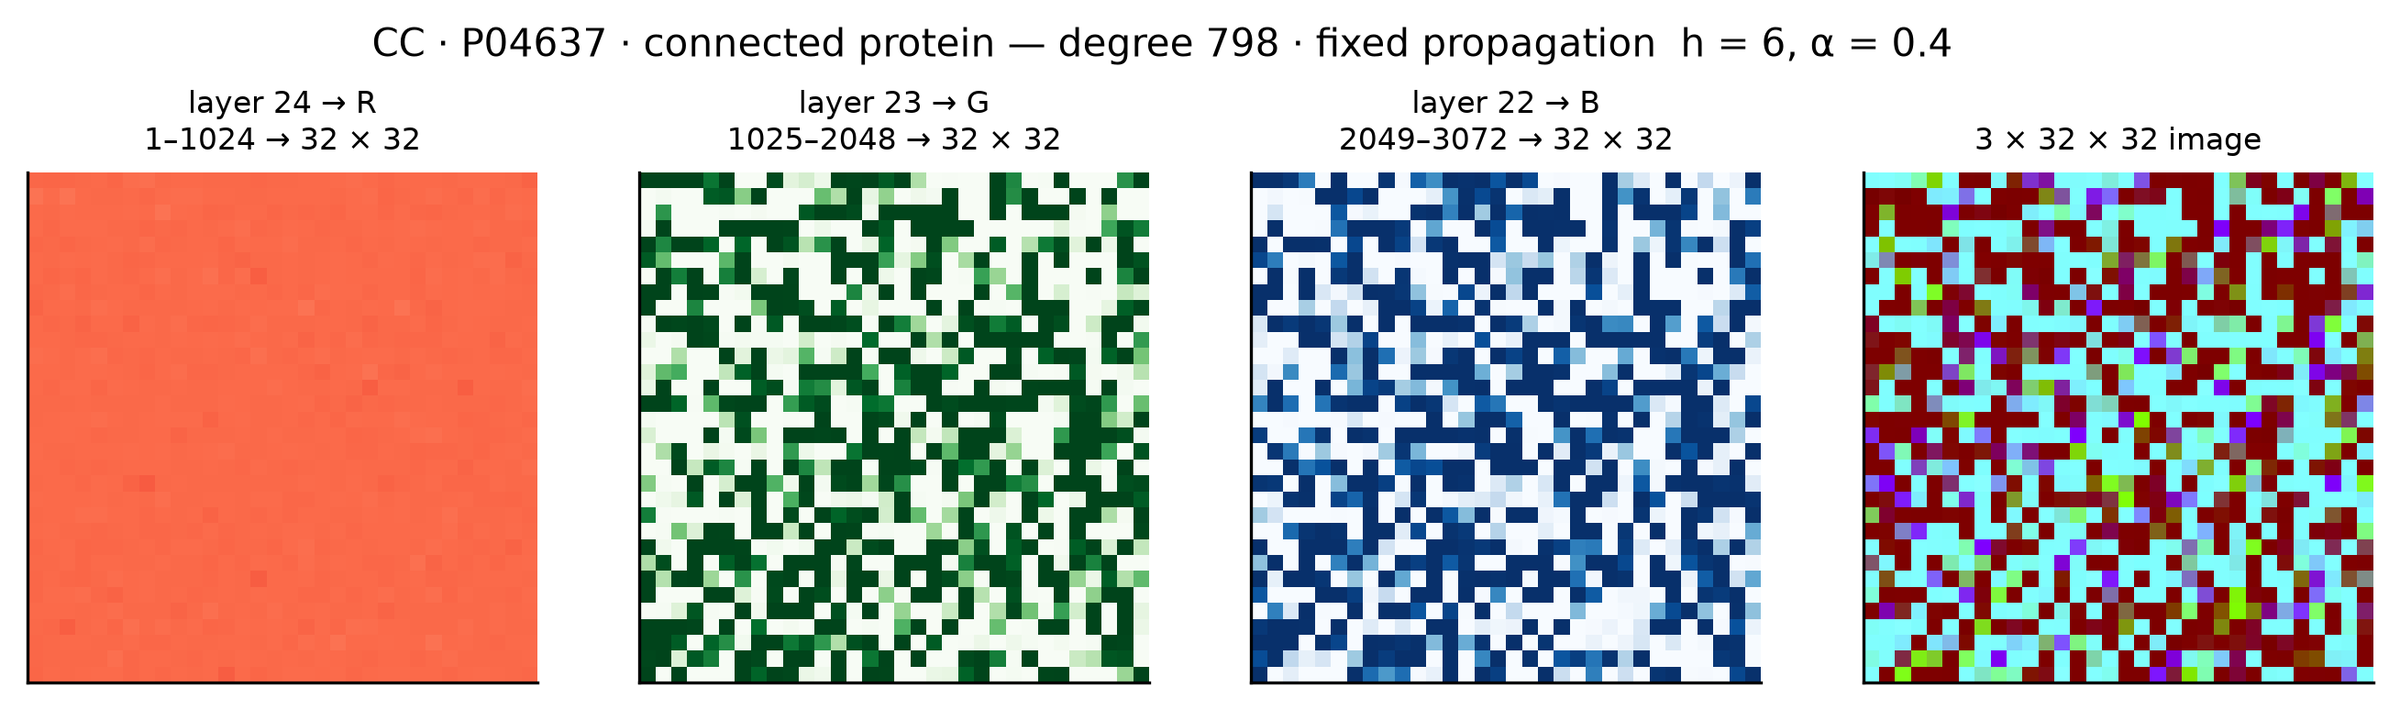
\includegraphics[height=0.3\textheight]{fig_5_9}
    \caption{De um vetor de 3.072 dimensões a uma imagem $32\times32\times3$.}
  \end{figure}
\end{frame}

\begin{frame}{Objetivo de Treinamento: ProteinLoss}
  \begin{eqbox}[0.7\textwidth]
    $\displaystyle \mathcal{L} = \mathcal{L}_{\mathrm{ZLPR}}\cdot\big(1-wF1^{\mathrm{GO}}\big)\cdot\big(1-wF1^{\mathrm{prot}}\big)$
  \end{eqbox}
  \begin{itemize}\setlength{\itemsep}{0.45em}
    \item A ZLPR~\cite{su2022zlpr} separa os termos positivos dos negativos no limiar zero
    \item Dois fatores $F_1$ suaves, ponderados por IC: um entre termos, outro entre proteínas~\cite{liu2024interlabelgo}
    \item Aproxima o treinamento do critério de avaliação
  \end{itemize}
\end{frame}

\begin{frame}{Combinando as Rotas Fixa e Aprendida}
  \begin{columns}[c]
    \column{0.44\textwidth}
    \begin{figure}
      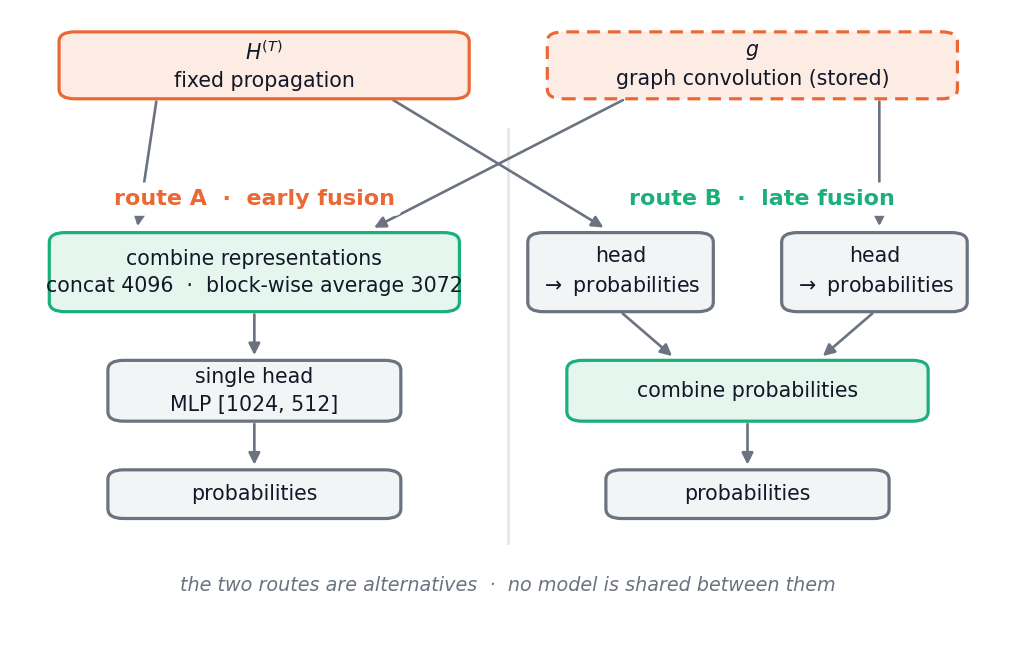
\includegraphics[width=\linewidth]{fig_5_10}
      \caption{Fusão precoce (esquerda) e fusão tardia (direita).}
    \end{figure}
    \column{0.54\textwidth}
    \begin{itemize}\setlength{\itemsep}{0.35em}\small
      \item \textbf{Fusão precoce:} une as representações e treina uma cabeça (concatenação 4.096 ou soma por blocos 3.072)
      \item \textbf{Fusão tardia:} treina cada rota e combina as probabilidades
      \item \textbf{Onze regras tardias:} $\gamma$ linear, máximo, mínimo, sigmoide de IC, sigmoide de grau, equação mestra e
        cinco metaclassificadores de empilhamento (\textit{stacking})
      \item Coeficientes escolhidos na validação (71 configurações por ontologia)
    \end{itemize}
  \end{columns}
\end{frame}

% =================================================================================== Results
\section{Resultados e Discussão}

\begin{frame}{Configuração Experimental}
  \begin{itemize}\setlength{\itemsep}{0.3em}
    \item \textbf{Execuções:} 170 execuções, cerca de 136,3 horas de GPU (147 delas numa RTX A5500)
    \item \textbf{Funil:} cada etapa escolhe sua vencedora na validação e a passa adiante; o teste é lido uma vez
    \item \textbf{Leitura:} semente única, então diferenças abaixo de 0,5\,p.p. são empates
  \end{itemize}
  \vspace{0.5em}
  \begin{table}\scriptsize
    \caption{A ordem das decisões e a vencedora de cada etapa.}
    \begin{tabular}{@{}lllll@{}}\toprule
      função de perda & arquitetura vetorial & \textit{backbone} visual & profundidade $T$ & retenção $\alpha$\\
      ProteinLoss & MLP \textit{raw} & ConvNeXt-Tiny & por ontologia & por ontologia\\\midrule
      codificador aprendido & deduplicação & fusão precoce & fusão tardia & teste\\
      GCN & max & soma + GCN + vetorial & $\gamma$ linear & \NX{Late}\\\bottomrule
    \end{tabular}
  \end{table}
\end{frame}

\begin{frame}{A Geração 1 Resolve Três Escolhas}
  \begin{table}\small
    \caption{Escolhas da Geração 1, $\wF$ médio na validação.}
    \begin{tabular}{@{}lll@{}}\toprule
      Escolha & Opção & $\wF$ médio \\ \midrule
      Piso & \textit{baseline} ingênuo de frequência de termos & 43,56 \\
      Função de perda & ProteinLoss contra entropia cruzada binária & +5,47\,p.p. (+8,87 em MF) \\
      Arquitetura vetorial & MLP sobre o perfil bruto & \textbf{44,51} \\
       & melhor CNN 1-D & 41,16 \\
      \textit{Backbone} visual & ResNet-50 e ConvNeXt-Tiny & de 36,99 a 37,62 \\ \bottomrule
    \end{tabular}
  \end{table}
  \vspace{0.5em}
  \begin{block}{Leitura}
    A topologia sozinha mal supera um preditor que não olha para nada: +0,95\,p.p. na média.
  \end{block}
\end{frame}

\begin{frame}{Profundidade e Retenção: Cabeça Vetorial}
  \begin{columns}[c]
    \column{0.49\textwidth}
    \begin{figure}
      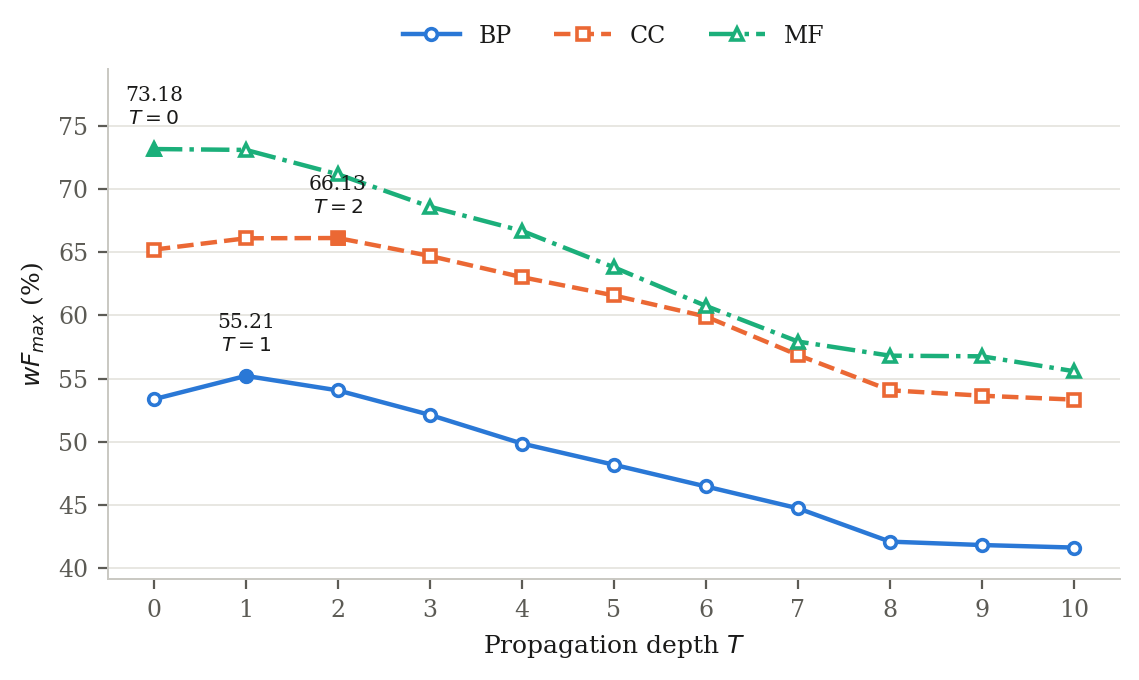
\includegraphics[width=\linewidth]{fig_6_1}
      \caption{Profundidade de propagação $T$.}
    \end{figure}
    \column{0.49\textwidth}
    \begin{figure}
      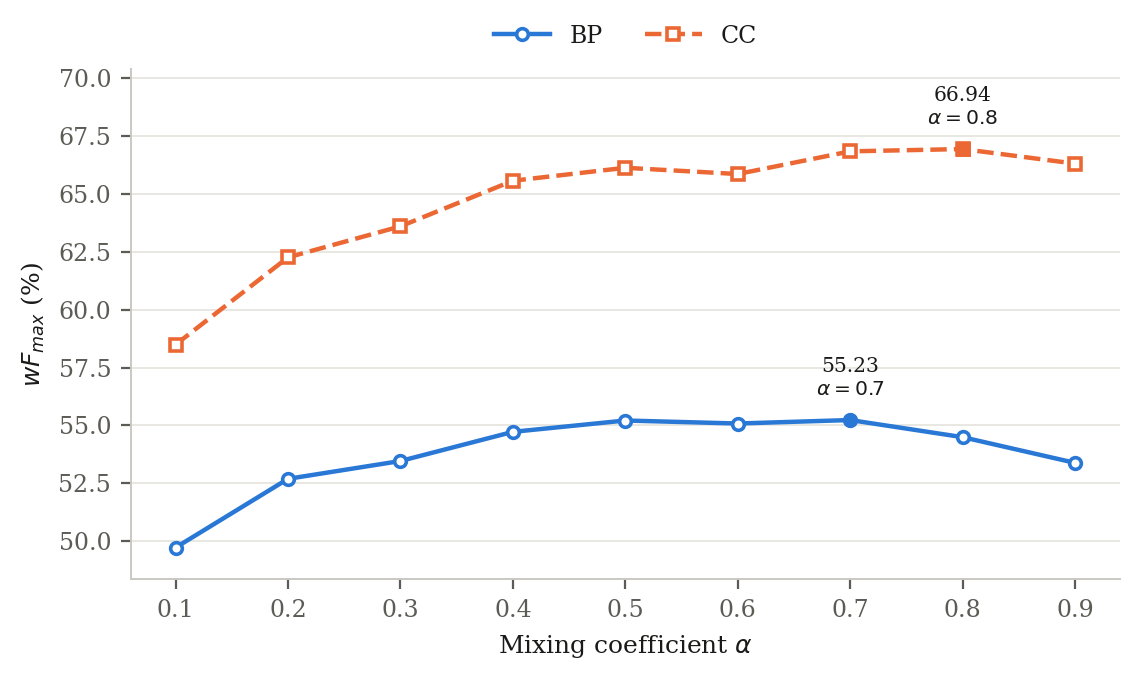
\includegraphics[width=\linewidth]{fig_6_2}
      \caption{Coeficiente de retenção $\alpha$.}
    \end{figure}
  \end{columns}
  \begin{itemize}\small
    \item \textbf{Pico:} $T=1$ em BP, $T=2$ em CC, $T=0$ em MF; até $T=10$, perdas de 12,80 a 17,60\,p.p.
    \item \textbf{Melhor retenção:} $\alpha=0{,}7$ em BP, $\alpha=0{,}8$ em CC; o grafo corrige a representação da proteína
  \end{itemize}
\end{frame}

\begin{frame}{Profundidade e Retenção: Cabeça Visual}
  \begin{columns}[c]
    \column{0.49\textwidth}
    \begin{figure}
      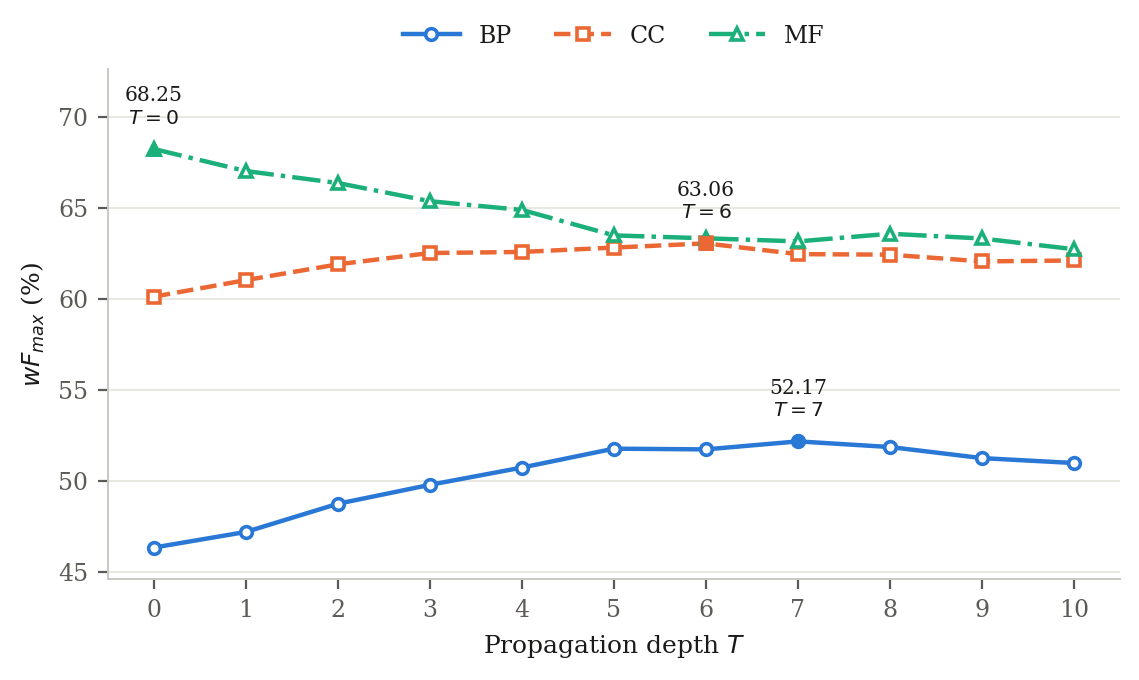
\includegraphics[width=\linewidth]{fig_6_3}
      \caption{Profundidade de propagação $T$.}
    \end{figure}
    \column{0.49\textwidth}
    \begin{figure}
      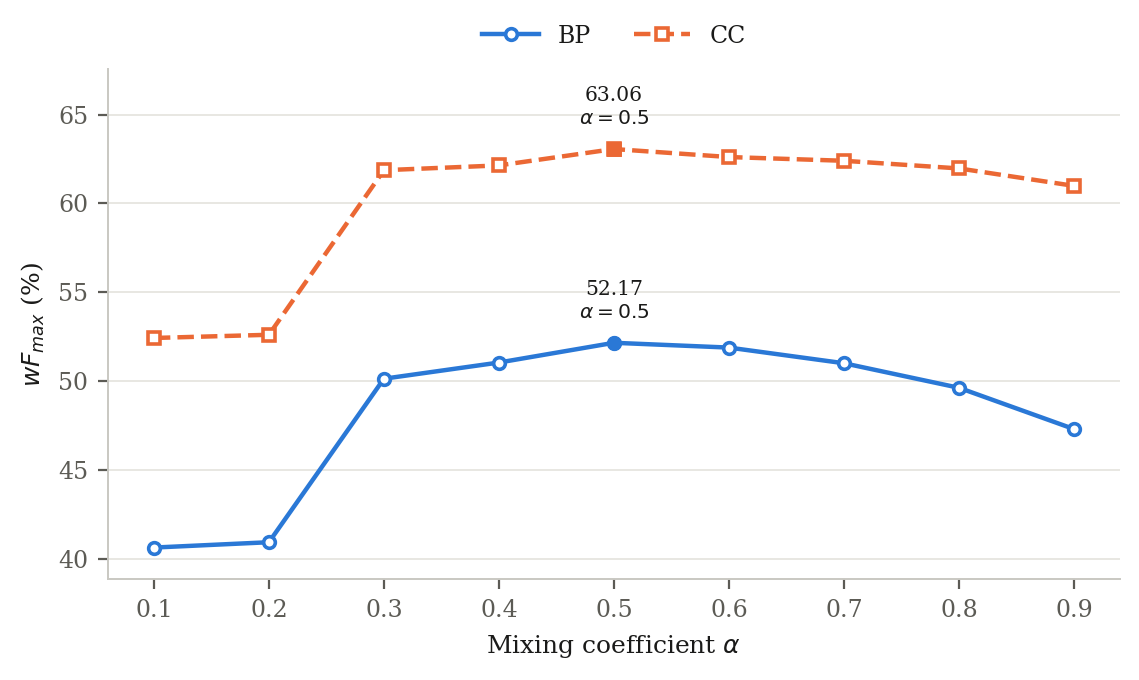
\includegraphics[width=\linewidth]{fig_6_4}
      \caption{Coeficiente de retenção $\alpha$.}
    \end{figure}
  \end{columns}
  \begin{itemize}\small
    \item \textbf{Pico:} $T=7$ em BP, $T=6$ em CC, $T=0$ em MF; ganhos sobre $T=0$: +5,84 em BP e +2,93 em CC (vetorial: +1,85
      e +0,92)
    \item Seu melhor valor em BP, 52,17, ainda fica abaixo dos 53,36 da cabeça vetorial sem grafo
  \end{itemize}
\end{frame}

\begin{frame}{Agregação Fixa ou Aprendida?}
  \begin{columns}[T]
    \column{0.64\textwidth}
    \begin{table}
      \caption{Rotas GNN de ponta a ponta, $\wF$ na validação.}
      \resizebox{\linewidth}{!}{\TabGNN}
    \end{table}
    \begin{itemize}\setlength{\itemsep}{0.3em}\small
      \item A GCN supera a GAT nos 6 pares (de 3,88 a 9,31\,p.p.) e em 30 de 30 pares de fusão
      \item \textbf{Deduplicação:} max nunca perde além do ruído; a GAT é a que mais ganha (+3,83 visual)
    \end{itemize}
    \column{0.34\textwidth}
    \vspace{1.2em}
    \only<2>{\callout{A propagação fixa chega a 65,12 de $\wF$ médio, contra 63,32 da GCN: a GCN
      lidera em BP por 0,55 (no limite do piso de 0,5\,p.p.) e fica atrás em CC por 0,59 e em MF por 5,35.}}
  \end{columns}
\end{frame}

\begin{frame}{A Fusão Ajuda; Combinar Predições Ajuda Mais}
  \begin{columns}[T]
    \column{0.52\textwidth}
    \begin{table}
      \caption{Regras de fusão tardia, $\wF$ na validação.}
      \resizebox{\linewidth}{!}{\TabLate}
    \end{table}
    \column{0.46\textwidth}
    \vspace{0.8em}
    \begin{itemize}\setlength{\itemsep}{0.35em}\small
      \item \textbf{Fusão precoce}, uma configuração (soma, GCN, vetorial): 65,80 (+0,68 sobre a fixa)
      \item \textbf{Fusão tardia}, $\gamma$ linear (0,50 BP, 0,55 CC e MF): 67,06, a melhor em toda ontologia
      \item Ganhos sobre o melhor componente: +2,18 BP, +1,85 CC e +1,26 MF
    \end{itemize}
    \vspace{0.5em}
    \only<2>{\callout{No empilhamento, as probabilidades das duas rotas levam quase todo o peso.}}
  \end{columns}
\end{frame}

\begin{frame}{A Cabeça Vetorial Vence 12 de 12}
  \begin{columns}[T]
    \column{0.64\textwidth}
    \begin{table}
      \caption{Cabeças vetorial e visual em cada etapa, $\wF$ na validação.}
      \resizebox{\linewidth}{!}{\TabVV}
    \end{table}
    \column{0.34\textwidth}
    \vspace{1.2em}
    \begin{itemize}\small
      \item \textbf{Margem na média:} +6,62, +3,96, +2,69 e +3,35\,p.p. nas quatro etapas, sem tendência a zero
    \end{itemize}
    \vspace{0.5em}
    \only<2>{\callout{Nenhuma das imagens tem a localidade que uma convolução pressupõe: a cabeça vetorial vence em toda
      etapa e ontologia.}}
  \end{columns}
\end{frame}

\begin{frame}{De Onde Vêm os Ganhos}
  \begin{center}
  \begin{tikzpicture}[x=1.85cm, y=0.12cm, font=\small]
    \draw[gray!60] (0.4,43) -- (7.6,43);
    \foreach \i/\v/\c/\l/\vt in \GainBars {
      \fill[\c] (\i-0.3,43) rectangle (\i+0.3,\v);
      \node[above, font=\scriptsize] at (\i,\v) {\vt};
      \node[below, font=\scriptsize] at (\i,43) {\l};
    }
  \end{tikzpicture}
  \end{center}
  {\scriptsize $\wF$ médio na validação; o eixo começa em 43. Azul: sequência; laranja: rede; verde: fusão.
  Early: melhor configuração por ontologia. A GNN sozinha fica abaixo do Só ProtT5 por causa de MF.}
  \begin{block}{Leitura}
    A maior parte do salto vem do modelo de linguagem; o grafo acrescenta o resto.
  \end{block}
\end{frame}

\begin{frame}{Conjunto de Teste: Comparação com a Literatura (BP)}
  \begin{columns}[T]
    \column{0.66\textwidth}
    \begin{table}\scriptsize
      \caption{Conjunto de teste, Processo Biológico.}
      \resizebox{\linewidth}{!}{\TabTestBP}
    \end{table}
    \column{0.32\textwidth}
    \vspace{1.5em}
    \begin{overprint}
      \onslide<2>\callout{\NX{Late} supera o \textit{baseline} mais forte, DeepGraphGO, por 9,77\,p.p. de $\wF$; o $\Smin$
        confirma: 17,12 contra 20,11 bits.}
      \onslide<3>\callout{O \textit{baseline} ProtT5 sozinho já supera todos os métodos da literatura em $\wF$.}
      \onslide<4>\callout{A propagação fixa acrescenta 1,87\,p.p. ao \textit{baseline} ProtT5: o grafo corrige a representação
        da sequência.}
    \end{overprint}
  \end{columns}
\end{frame}

\begin{frame}{Conjunto de Teste: Comparação com a Literatura (CC)}
  \begin{columns}[T]
    \column{0.66\textwidth}
    \begin{table}\scriptsize
      \caption{Conjunto de teste, Componente Celular.}
      \resizebox{\linewidth}{!}{\TabTestCC}
    \end{table}
    \column{0.32\textwidth}
    \vspace{1.5em}
    \begin{overprint}
      \onslide<2>\callout{\NX{Late} supera o \textit{baseline} mais forte, DeepGraphGO, por 8,67\,p.p. de $\wF$; o $\Smin$
        confirma: 8,22 contra 9,67 bits.}
      \onslide<3>\callout{A Primeira Geração, só de topologia, fica 16,39\,p.p. abaixo do \textit{baseline} ProtT5: a
        maior parte do ganho vem do modelo de linguagem.}
      \onslide<4>\callout{A propagação fixa acrescenta 2,15\,p.p. ao \textit{baseline} ProtT5: o grafo complementa a sequência.}
    \end{overprint}
  \end{columns}
\end{frame}

\begin{frame}{Conjunto de Teste: Comparação com a Literatura (MF)}
  \begin{columns}[T]
    \column{0.66\textwidth}
    \begin{table}\scriptsize
      \caption{Conjunto de teste, Função Molecular.}
      \resizebox{\linewidth}{!}{\TabTestMF}
    \end{table}
    \column{0.32\textwidth}
    \vspace{1.5em}
    \begin{overprint}
      \onslide<2>\callout{\NX{Late} supera o \textit{baseline} mais forte, DeepGraphGO, por 4,93\,p.p. de $\wF$; o $\Smin$
        confirma: 5,14 contra 5,67 bits.}
      \onslide<3>\callout{O \textit{baseline} ProtT5 e o \NX{Fixed} são a mesma execução: em MF, a melhor profundidade é $T=0$.
        Em $\wF$, só as rotas de fusão superam essa execução, e por pouco.}
      \onslide<4>\callout{Nas três ontologias, o \NX{Late} é o melhor em todas as colunas, exceto AuPRC em MF, em que o
        \NX{Early} lidera por 5,35\,p.p.}
    \end{overprint}
  \end{columns}
\end{frame}

\begin{frame}{Toda Proteína Recebe uma Predição}
  \begin{table}\small
    \caption{Cobertura de predição na partição de teste, por família de métodos.}
    \TabCov
  \end{table}
  \begin{itemize}\setlength{\itemsep}{0.35em}
    \item DeepGraphGO e SEGT-GO alcançam proteínas fora da rede por busca de homologia
    \item Mashup, MELISSA e deepNF só pontuam membros da rede; as ausentes contam como erros
    \item Parte da distância para os métodos só de rede é alcance, não qualidade do ranqueamento
  \end{itemize}
\end{frame}

\begin{frame}{Custo Computacional}
  \begin{columns}[c]
    \column{0.5\textwidth}
    \begin{figure}
      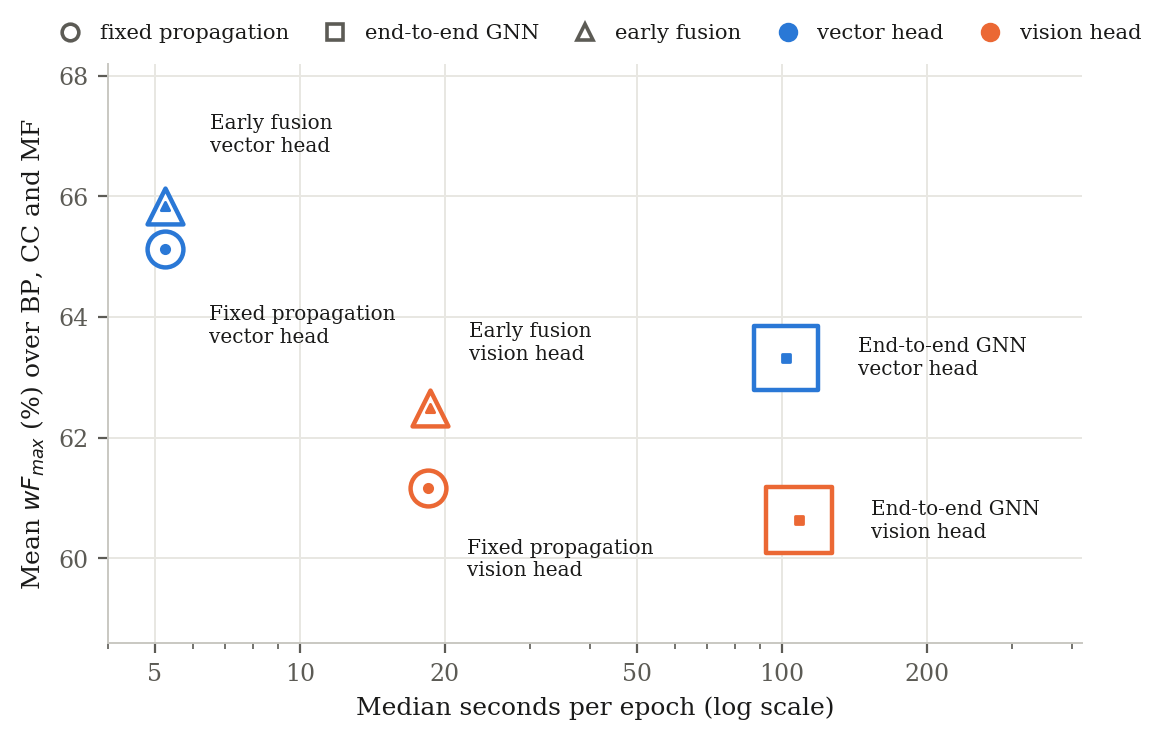
\includegraphics[width=\linewidth]{fig_6_5}
      \caption{$\wF$ médio contra a mediana de segundos por época (escala log).}
    \end{figure}
    \column{0.48\textwidth}
    \begin{itemize}\setlength{\itemsep}{0.35em}\small
      \item \textbf{Fixa + vetorial:} 5,24\,s/época, pico de 6,4\,GiB
      \item \textbf{Só a GCN:} 68,76\,s/época e 14,1\,GiB; GAT: 161,41\,s e 20,7\,GiB
      \item Iguala ou supera a GCN com cerca de 1/13 do tempo e menos da metade da memória
      \item A fusão precoce custa o mesmo que a propagação fixa quando $g$ já está armazenado
    \end{itemize}
  \end{columns}
\end{frame}

\begin{frame}{O Grafo Ajuda Onde Há Grafo}
  \begin{columns}[c]
    \column{0.54\textwidth}
    \begin{figure}
      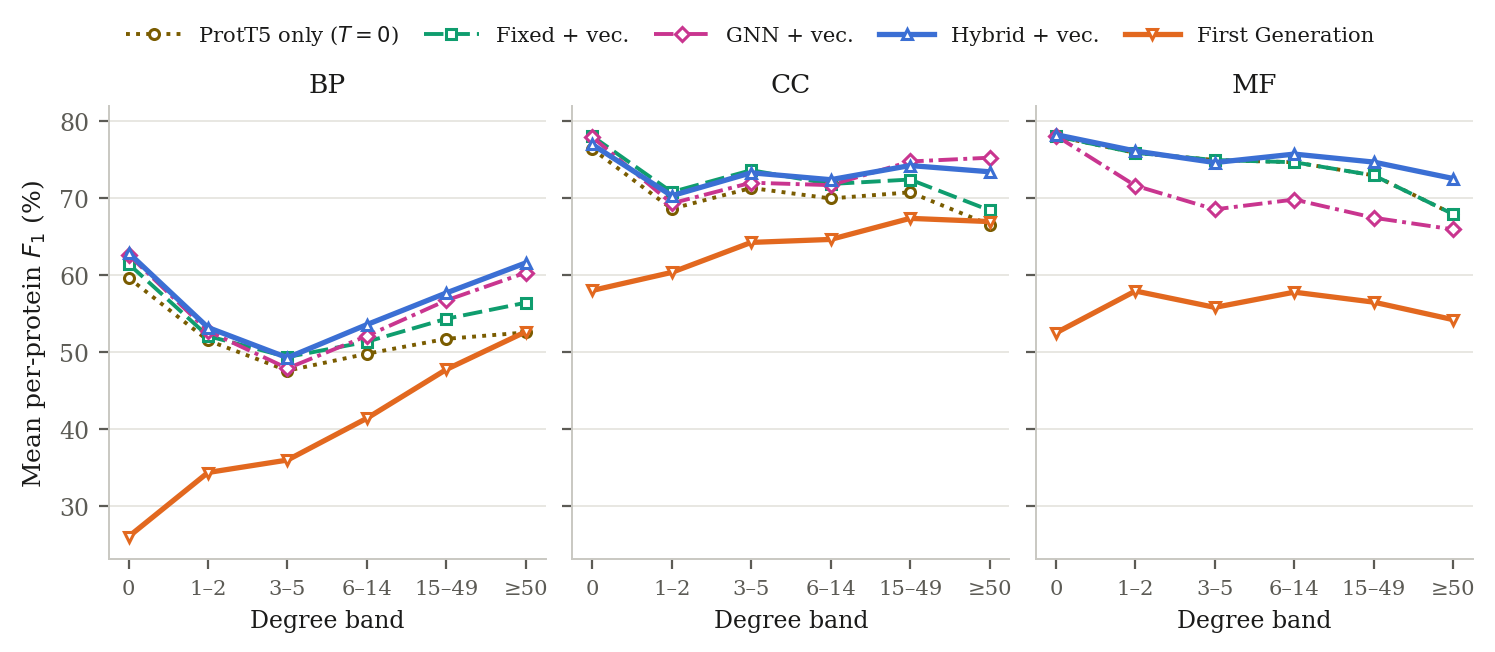
\includegraphics[width=\linewidth]{fig_6_6}
      \caption{$F_1$ por proteína e faixa de grau, conjunto de teste.}
    \end{figure}
    \column{0.44\textwidth}
    \begin{table}
      \caption{Ganho sobre o controle $T=0$ ($F_1$ por proteína, teste, p.p.); f fixa, g GNN, h fusão precoce.}
      \resizebox{\linewidth}{!}{\TabGain}
    \end{table}
  \end{columns}
  \begin{itemize}\small
    \item Toda rota com ProtT5 pontua pior nas conectadas que nas isoladas, como o controle sem grafo
    \item O ganho do grafo cresce com o grau: até +9,05 BP, +8,71 CC e +4,64 MF com grau $\ge 50$
  \end{itemize}
\end{frame}

% =================================================================================== Conclusions
\section{Conclusões e Contribuições}

\begin{frame}{Conclusões Gerais}
  \begin{itemize}\setlength{\itemsep}{0.45em}\small
    \item \textbf{Primeiro o modelo de linguagem:} a maior parte do ganho vem do ProtT5 (44,51 só com a rede e 63,92
      só com o ProtT5, em $\wF$ médio na validação); o grafo acrescenta o resto.
    \item \textbf{Fixa equivale à aprendida:} a propagação fixa (65,12) iguala ou supera a GCN (63,32) com cerca de 1/13
      do tempo por época.
    \item \textbf{A fusão compensa:} a fusão tardia chega a 67,06, a melhor em toda ontologia (validação).
    \item \textbf{Cabeça vetorial:} vence 12 de 12 comparações; as imagens impõem uma localidade que os dados não têm.
    \item \textbf{O grafo ajuda onde há grafo:} o ganho cresce com o grau, até +9,05\,p.p. em BP.
  \end{itemize}
\end{frame}

\begin{frame}{Respostas às Questões de Pesquisa (1/4)}
  \begin{itemize}\setlength{\itemsep}{0.9em}\small
    \item<+-> \textbf{(QP1)} {\scriptsize\textit{Como diferentes representações dos dados da rede PPI do STRING afetam a qualidade da predição de função nos três domínios da GO?}}\\[0.2em]
      A representação e o seu viés indutivo pesam muito. O perfil de escores sem redução lidera as alternativas com \textit{pooling} por até 4,53\,p.p. na média das três ontologias, e as arquiteturas que impõem ordem 1-D ou localidade 2-D a coordenadas que são proteínas de treino em ordem arbitrária pioram nos três domínios.
    \item<+-> \textbf{(QP2)} {\scriptsize\textit{Em que medida a propagação fixa dos \textit{embeddings} do ProtT5 pela rede STRING melhora a representação só de rede, e como esse efeito varia entre BP, MF e CC?}}\\[0.2em]
      O ganho é grande, mas vem sobretudo do \textit{embedding} de sequência. No teste, a rota só de rede fica 16,44 (BP), 16,39 (CC) e 23,95\,p.p. (MF) abaixo do controle ProtT5 sem grafo; a propagação acrescenta +1,87 em BP e +2,15 em CC sobre esse controle, e nada em MF, onde a profundidade ótima é zero. O grafo corrige a representação; não a substitui.
  \end{itemize}
\end{frame}

\begin{frame}{Respostas às Questões de Pesquisa (2/4)}
  \begin{itemize}\setlength{\itemsep}{0.9em}\small
    \item<+-> \textbf{(QP3)} {\scriptsize\textit{Como se comparam estratégias que vão de \textit{embeddings} de grafo simples à propagação fixa não paramétrica e às GNNs, sob um protocolo experimental comum e com cabeças de classificação vetorial e visual?}}\\[0.2em]
      Pelo $\wF$ médio na validação: Late 67,06 $>$ Early 65,84 $>$ Fixed 65,12 $>$ GNN 63,32. Os métodos de \textit{embedding} de grafo da literatura ficam abaixo do prior de frequência de termos em ao menos um domínio, e a ordem se mantém com cada cabeça; a vetorial vence a visual em 12 de 12 comparações.
    \item<+-> \textbf{(QP4)} {\scriptsize\textit{As fusões precoce e tardia melhoram a métrica principal em relação aos seus componentes de propagação fixa e de GNN?}}\\[0.2em]
      As duas ajudam, e combinar predições ajuda mais que combinar representações. A Early ganha 0,72\,p.p. na média sobre a melhor das representações que funde. A Late ganha +2,18 em BP, +1,85 em CC e +1,26 em MF sobre o melhor componente; um único escalar supera cinco metaclassificadores de \textit{stacking}, ao custo de um parâmetro ajustado na validação.
  \end{itemize}
\end{frame}

\begin{frame}{Respostas às Questões de Pesquisa (3/4)}
  \begin{itemize}\setlength{\itemsep}{0.9em}\small
    \item<+-> \textbf{(QP5)} {\scriptsize\textit{Como a profundidade da propagação e o coeficiente de retenção afetam o desempenho, e a partir de que ponto propagar mais começa a diluir o sinal da própria proteína?}}\\[0.2em]
      Com a cabeça vetorial, o ótimo fica em um ou dois saltos, e a diluição começa logo depois: o desempenho cai 13,60 (BP), 12,80 (CC) e 17,60\,p.p. (MF) entre o pico e dez saltos. Em BP e CC, a retenção domina, com $\alpha$ ótimo entre 0,7 e 0,8; em MF a profundidade ótima é zero. Uma proteína sem vizinhos só é multiplicada por $\alpha^{T}$.
    \item<+-> \textbf{(QP6)} {\scriptsize\textit{Como a abordagem proposta se compara a algoritmos de referência baseados em rede, com todos os métodos avaliados nas mesmas partições e no mesmo cenário transdutivo?}}\\[0.2em]
      A \NX{Late} tem o melhor valor de todas as colunas das três tabelas de confronto, com uma exceção: AuPRC em MF, em que a Early fica à frente. A margem sobre o \textit{baseline} mais forte é de +9,77 (BP), +8,67 (CC) e +4,93\,p.p. (MF) de $\wF$ no teste, e o $\Smin$ concorda.
  \end{itemize}
\end{frame}

\begin{frame}{Respostas às Questões de Pesquisa (4/4)}
  \begin{itemize}\setlength{\itemsep}{0.9em}\small
    \item<+-> \textbf{(QP7)} {\scriptsize\textit{A metodologia funciona aplicada diretamente a redes globais de evidências agregadas (várias fontes de interação e várias espécies numa única topologia), sem particionar o grafo por espécie ou por canal de evidência?}}\\[0.2em]
      Sim: o NEXUS-GO opera numa rede global e multiespécie, com os canais de evidência já agregados, sem etapa de particionamento, e alcança o maior $\wF$ da comparação; as configurações pensadas para várias redes separadas, entre elas o deepNF, são as que pior se saem nela. Isso mostra aplicabilidade, não superioridade sobre particionar por espécie ou por canal: esse contrafactual não foi executado.
  \end{itemize}
\end{frame}

\begin{frame}{Limitações do Estudo}
  \begin{itemize}\setlength{\itemsep}{0.45em}
    \item \textbf{Semente única:} o piso de 0,5\,p.p. é uma convenção de leitura, não um intervalo de confiança
    \item Partição aleatória por proteína: interpolação transdutiva, possível vazamento por homologia
    \item Os escores do STRING podem codificar conhecimento de anotação (circularidade)
    \item Fixa contra aprendida não é uma ablação de fator único (escala $\alpha^{T}$, normalização)
    \item \textit{Baselines} adaptados a uma única rede agregada e a um espaço de rótulos reduzido
  \end{itemize}
\end{frame}

\begin{frame}{Trabalhos Futuros}
  \begin{itemize}\setlength{\itemsep}{0.45em}
    \item Separar o grafo por organismo, ou treinar um modelo por organismo
    \item Manter separados os canais de evidência do STRING (arestas tipadas ou paralelas)
    \item Grafos heterogêneos de proteínas, termos e evidências; comparar com o ProtHGT~\cite{ulusoy2025prothgt}
    \item Agregação por amostragem (GraphSAGE~\cite{hamilton2017graphsage}) para uma rota aprendida mais barata
    \item Atributos de nó mais ricos: estrutura, domínios, expressão; o mais promissor para MF
  \end{itemize}
\end{frame}

\begin{frame}{Contribuições e Publicações}
  \textbf{Contribuições científicas:}
  \begin{itemize}\setlength{\itemsep}{0.15em}\small
    \item \textbf{Método:} NEXUS-GO, uma propagação não paramétrica de múltiplos saltos de \textit{embeddings} do ProtT5 pelo
      STRING
    \item \textbf{Comparações controladas:} agregação fixa contra aprendida (GCN, GAT); cabeça vetorial contra visual
    \item \textbf{Fusão:} fusão precoce e tardia das duas rotas; a fusão tardia linear dá o melhor $\wF$ do trabalho
    \item \textbf{\textit{Benchmark}:} cinco métodos baseados em redes, retreinados nas mesmas partições e no mesmo cenário
      transdutivo
  \end{itemize}
  \vspace{0.3em}
  \textbf{Produção acadêmica:}
  \begin{itemize}\setlength{\itemsep}{0.15em}\small
    \item Artigo publicado no \textbf{VISAPP 2026} (Marbella, Espanha)~\cite{mauhnoom2026graphs}
    \item Versão estendida aceita na série \textbf{Communications in Computer and Information Science}, prevista para
      dezembro de 2026~\cite{mauhnoom2026beyond}
    \item Código: \texttt{github.com/ymauhn/nexus-go}
  \end{itemize}
\end{frame}

\begin{frame}[allowframebreaks]{Referências}
  \scriptsize
  % the entries are in English: English hyphenation keeps the four frames of the English deck
  \begin{otherlanguage}{english}
  \bibliographystyle{abbrv}
  \bibliography{references}
  \end{otherlanguage}
\end{frame}

\begin{frame}{Agradecimentos}
  \begin{itemize}\setlength{\itemsep}{0.35em}\small
    \item Ao meu orientador, Prof.\ Dr.\ Zanoni Dias, e aos meus coorientadores, Prof.\ Dr.\ Hélio Pedrini e Dr.\
      Gabriel Bianchin de Oliveira, pela orientação
    \item À minha família, em especial aos meus pais, e aos meus amigos e colegas, pelo apoio
    \item À CAPES e ao BTG Pactual, pelo apoio financeiro
    \item Ao Instituto de Computação da Unicamp, pelos recursos computacionais
  \end{itemize}
  \vfill
  \begin{columns}[c]
    \column{0.5\textwidth}\centering
    
\includegraphics[height=2.0cm]{logo-unicamp}\\[0.3em]
    {\small Universidade Estadual de Campinas (Unicamp)}
    \column{0.5\textwidth}\centering
    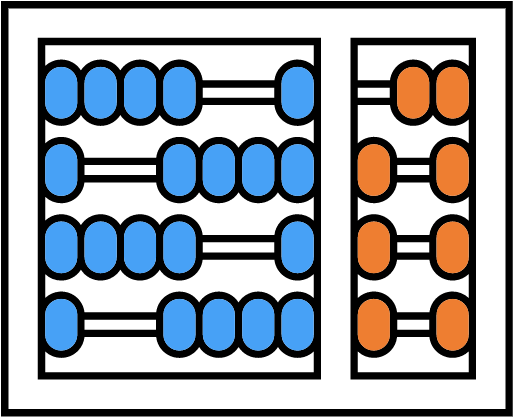
\includegraphics[height=1.6cm]{logo-ic}\\[0.5em]
    {\small Instituto de Computação (IC)}
  \end{columns}
  \vfill
\end{frame}

\begin{frame}
  \titlepage
\end{frame}

% =================================================================================== Backup
\appendix
\section*{Backup}

\begin{frame}{Backup: Custo Computacional por Família}
  \begin{table}\scriptsize
    \caption{RTX A5500, 147 execuções; menor valor em negrito para s/época, h/execução e VRAM.}
    \TabCost
  \end{table}
\end{frame}

\begin{frame}{Backup: Deduplicação dos Registros do STRING}
  \begin{itemize}\setlength{\itemsep}{0.45em}
    \item Pesos simétricos, sem laços, armazenamento COO esparso (até 1,13 milhão de entradas armazenadas; a matriz
      densa ocuparia de 25 a 35\,GB)
    \item \textbf{max} preserva o escore; a \textbf{soma} o multiplica pelo número de registros
  \end{itemize}
  \begin{block}{Exemplo}
    Vizinho A (escore 0,80, com 5 registros) e B (0,95, com 1 registro). Com a soma, A pesa 4,00 contra 0,95 e domina;
    com o max, B (0,95) fica acima de A (0,80). A normalização não desfaz a reordenação.
  \end{block}
\end{frame}

\end{document}
